% Capitolo 6: Risultati e discussione

In questo capitolo si presentano i risultati ottenuti con il polarimetro a immagine. L'esposizione segue l'ordine logico della validazione: si parte da una panoramica qualitativa dei dati prodotti dal sistema su un campione fotoelastico di prova, si passa ai test di accuratezza su campioni a ritardanza nota (le lamine d'onda), alla verifica della linearità della risposta su un campione a ritardanza crescente (il nastro stratificato), e infine alla dimostrazione della versatilità del sistema su fenomeni di natura distinta, l'attività ottica e la fotoelasticità sotto carico.

% ---------------------------------------------------------------------------
\section{Panoramica dei dati e validazione qualitativa}
\label{sec:panoramica_righello}

Il primo campione analizzato, e il banco di prova qualitativo iniziale del polarimetro, è un comune righello in materiale polimerico trasparente. I materiali plastici formati per stampaggio a iniezione conservano tensioni interne congelate nel processo di fabbricazione, che inducono una birifrangenza residua; osservata in luce polarizzata, questa si manifesta come un caratteristico pattern di frange fotoelastiche. Il campione non richiede preparazione né sollecitazione esterna, e la presenza immediata delle frange offre una verifica diretta che la catena di acquisizione e ricostruzione produce mappe polarimetriche sensate. Per questa ragione lo si presenta in apertura, sia come validazione qualitativa del funzionamento del sistema sia come panoramica del tipo di dato che il polarimetro restituisce.

Prima di procedere conviene fissare il riferimento di polarizzazione in ingresso. In ogni acquisizione lo sfondo libero attorno al campione, da cui la pipeline ricava il riferimento tramite il fit di superficie descritto nella \cref{sec:allineamento}, presenta $\mathrm{DoLP} \approx 1$, $\mathrm{AoLP} \approx 0^\circ$ e $S_3 \approx 0$, coerentemente con la luce linearmente polarizzata emessa dal display LCD. Lo sfondo non è mai stato acquisito in modo isolato, ma il fit sulla porzione visibile è ampiamente sufficiente a fissare tale riferimento, rispetto al quale sono misurate tutte le grandezze polarimetriche dei campioni.

La \cref{fig:righello_overview} riporta, sul canale rosso, le sei grandezze che riassumono lo stato di polarizzazione pixel per pixel: l'intensità totale $S_0$, le tre componenti normalizzabili $S_1$, $S_2$, $S_3$ del vettore di Stokes, il grado di polarizzazione lineare DoLP e l'angolo di polarizzazione lineare AoLP. L'insieme fornisce al lettore una prima panoramica del dato polarimetrico bidimensionale e del modo in cui un singolo fenomeno fisico si distribuisce fra i diversi parametri.

\begin{figure}[H]
    \centering
    \subfloat[$S_0$]{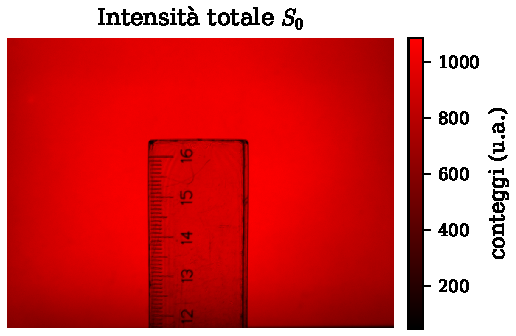
\includegraphics[height=0.205\textwidth]{Images/generated/righello_v2/R_S0.pdf}}\hfill
    \subfloat[$S_1$]{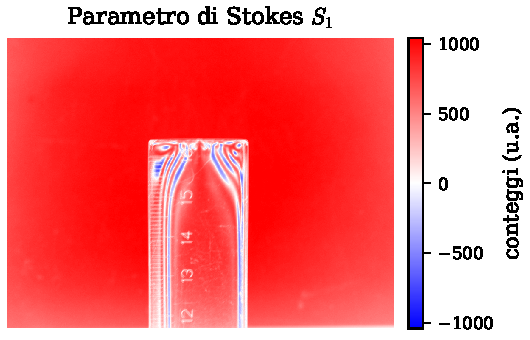
\includegraphics[height=0.205\textwidth]{Images/generated/righello_v2/R_S1.pdf}}\hfill
    \subfloat[$S_2$]{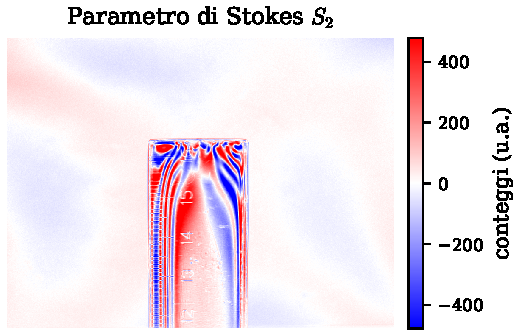
\includegraphics[height=0.205\textwidth]{Images/generated/righello_v2/R_S2.pdf}}\\
    \subfloat[$S_3$]{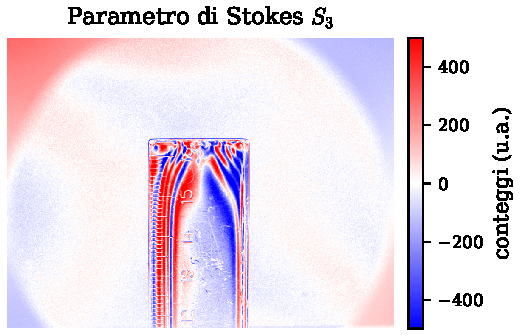
\includegraphics[height=0.205\textwidth]{Images/generated/righello_v2/R_S3.pdf}}\hfill
    \subfloat[DoLP]{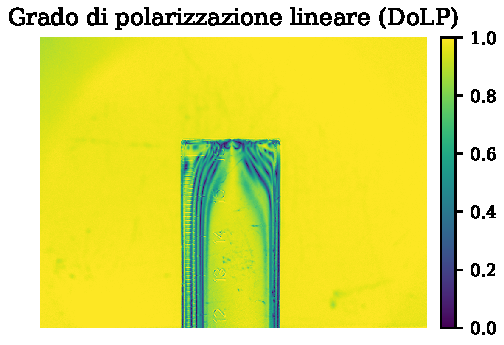
\includegraphics[height=0.205\textwidth]{Images/generated/righello_v2/R_DoLP.pdf}}\hfill
    \subfloat[AoLP]{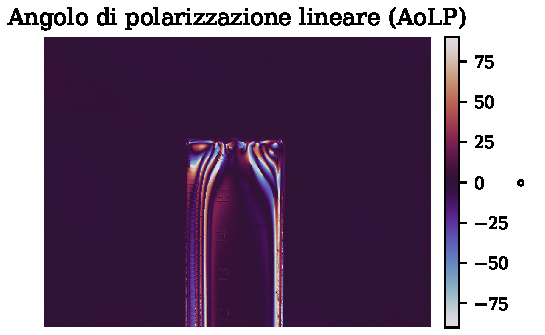
\includegraphics[height=0.205\textwidth]{Images/generated/righello_v2/R_AoLP.pdf}}
    \caption{Panoramica dei parametri polarimetrici per il righello in plastica trasparente, canale rosso. Le frange fotoelastiche dovute alle tensioni residue di stampaggio sono visibili nelle mappe di $S_1$, $S_2$ e in particolare del DoLP, dove le bande scure ($\mathrm{DoLP} \approx 0$) corrispondono ai punti in cui lo stato emergente è prossimo alla polarizzazione circolare (ritardanza pari a un multiplo dispari di $90^\circ$, con assi locali della birifrangenza a circa $45^\circ$ dalla polarizzazione incidente).}
    \label{fig:righello_overview}
\end{figure}

Le frange sono più leggibili nella mappa del DoLP: le bande scure, dove $\mathrm{DoLP} \approx 0$, segnano i luoghi in cui lo stato emergente è prossimo alla polarizzazione circolare, condizione che si realizza dove la ritardanza accumulata è un multiplo dispari di $90^\circ$ e gli assi locali della birifrangenza formano un angolo prossimo a $45^\circ$ con la polarizzazione incidente; dove la ritardanza è invece un multiplo intero di $\pi$ lo stato emergente torna linearmente polarizzato e il DoLP risale verso l'unità. La loro distribuzione spaziale ricalca l'andamento delle tensioni interne lungo il corpo del righello. Poiché la ritardanza dipende dalla lunghezza d'onda, lo stesso campo di sforzo produce frange più fitte alle lunghezze d'onda corte: la \cref{fig:righello_dolp_rgb} confronta la mappa del DoLP sui tre canali colore, e la frequenza spaziale delle frange cresce visibilmente dal rosso al blu, coerentemente con l'aumento della ritardanza al diminuire di $\lambda$.

\begin{figure}[H]
    \centering
    \subfloat[Canale R ($\lambda_\mathrm{eff} \approx \SI{626}{\nano\meter}$)]{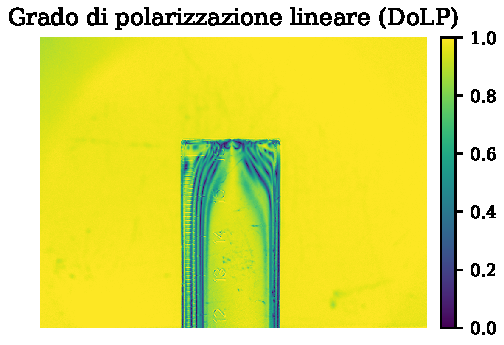
\includegraphics[height=0.205\textwidth]{Images/generated/righello_v2/R_DoLP.pdf}}\hfill
    \subfloat[Canale G ($\lambda_\mathrm{eff} \approx \SI{536}{\nano\meter}$)]{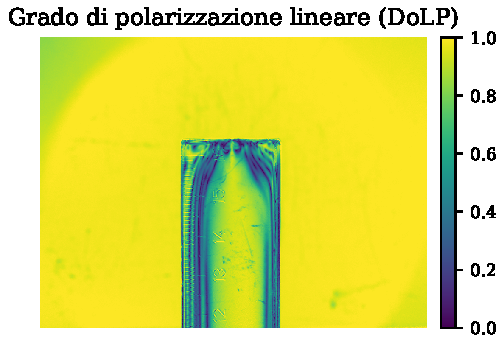
\includegraphics[height=0.205\textwidth]{Images/generated/righello_v2/G_DoLP.pdf}}\hfill
    \subfloat[Canale B ($\lambda_\mathrm{eff} \approx \SI{466}{\nano\meter}$)]{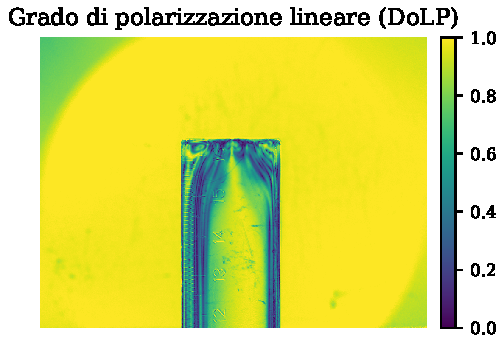
\includegraphics[height=0.205\textwidth]{Images/generated/righello_v2/B_DoLP.pdf}}
    \caption{Mappe del DoLP del righello sui tre canali del sensore. La frequenza spaziale delle frange fotoelastiche aumenta dal rosso al blu, manifestazione diretta della crescita della ritardanza al diminuire della lunghezza d'onda.}
    \label{fig:righello_dolp_rgb}
\end{figure}

L'esito è qualitativo ma significativo: senza alcuna calibrazione quantitativa il polarimetro restituisce mappe coerenti che rivelano la birifrangenza residua del materiale e la sua dipendenza spettrale, confermando il corretto funzionamento dell'intera catena di misura prima dei test di accuratezza presentati nelle sezioni successive.

% ---------------------------------------------------------------------------
\section{Calibrazione della correzione cromatica di \texorpdfstring{$S_3$}{S3}}
\label{sec:calibrazione_s3}

La ricostruzione di $S_3$ (\cref{eq:s3_formula}) contiene un unico parametro libero, il ritardo $\delta_a(\lambda)$ della lamina $\lambda/4$ impiegata come analizzatore, attraverso il fattore di correzione cromatica $1/\sin\delta_a(\lambda)$. Poiché ogni mappa di ritardanza e ogni mappa dell'asse veloce dei campioni birifrangenti dipendono da $S_3$, la scelta di $\delta_a(\lambda)$ condiziona l'intero capitolo. Adottarne un valore da un modello di materiale lascerebbe i risultati appesi a un'assunzione non verificata: il costruttore non dichiara né il materiale della lamina né il suo ordine. Si è perciò preferito \emph{misurare} $\delta_a(\lambda)$ direttamente dai dati, prima di applicare la pipeline ai campioni.

La misura sfrutta un'identità dell'apparato. La lamina $\lambda/4$ analizzata come campione nel dataset \texttt{lambdaquarti} è dello stesso tipo della lamina $\lambda/4$ inserita come analizzatore di $S_3$ in tutte le acquisizioni: le due condividono per costruzione lo stesso ritardo $\delta_a(\lambda)$. Misurare la ritardanza del campione equivale dunque a misurare la quantità che entra nella correzione. Il punto determinante è che questa misura può essere condotta senza ricorrere a $S_3$ e senza alcun modello di dispersione. I parametri lineari $S_0$, $S_1$, $S_2$ provengono dalle trentasei acquisizioni con il solo analizzatore lineare rotante, in cui la lamina $\lambda/4$ analizzatore non è presente nel cammino ottico; la ritardanza del campione vi è impressa attraverso la conversione dello stato di polarizzazione incidente, e il suo modulo è fissato dal canale coseno, costruito sui soli $S_0$, $S_1$, $S_2$. Il segno di $\delta_a$, e con esso il completamento a $[0^\circ, 360^\circ)$, non serve alla correzione, che dipende dal solo $\sin\delta_a$.

Resta da rendere la stima immune da due effetti che, se trascurati, la distorcerebbero. Il primo è la depolarizzazione introdotta dalla lamina, che riduce il grado di polarizzazione totale dal valore prossimo all'unità dello sfondo a circa $0{,}9$ nel rosso e $0{,}8$ nel blu: normalizzare sul livello dello sfondo, come fa il canale coseno, spinge artificiosamente la ritardanza verso $90^\circ$. Il secondo è l'ellitticità residua del fascio incidente, già rimossa nella pipeline dalla rotazione di Poincaré attorno all'asse $S_2$ (\cref{sec:ellitticita}). Entrambi si neutralizzano lavorando con i \emph{rapporti} fra le componenti del vettore di Stokes, ovvero con la sua direzione: sotto depolarizzazione scalare il fattore di depolarizzazione $p$ moltiplica tutte le componenti e si elide nei rapporti, lasciando inalterata la direzione dell'ellisse e quindi la ritardanza. La direzione del vettore, ricostruita sui pixel della lamina dopo gli allineamenti, fornisce così una stima di $\delta_a$ indipendente dalla normalizzazione di sfondo.

L'ultimo ingrediente chiude il problema senza introdurre circolarità. La differenza grezza $I_{-45} - I_{+45}$, non ancora divisa per $\sin\delta_a$, raccoglie due fattori $\sin\delta_a$: uno introdotto dalla lamina-campione nel convertire la polarizzazione, l'altro dall'analizzatore identico nel rivelarla. Vale pertanto, per uno stato incidente lineare di riferimento,
\begin{equation}
    I_{-45} - I_{+45} \;\propto\; p \, \sin 2\theta \, \sin^2\!\delta_a,
    \label{eq:s3_selfref}
\end{equation}
dove $\theta$ è l'orientazione dell'asse della lamina. Il ritardo $\delta_a$ vi compare al quadrato e si auto-riferisce: rapportando la \cref{eq:s3_selfref} alle componenti lineari $S_1$, $S_2$, nelle quali $p$ si elide, si ottiene un sistema di due equazioni nelle due incognite $\delta_a$ e $\theta$, risolto in modo auto-consistente con la rotazione di Poincaré effettivamente usata nella pipeline. La soluzione non assume alcun materiale, alcun ordine, né la correzione che si intende calibrare.

I valori così ottenuti sono riportati nella \cref{tab:s3_calibrazione}. La bontà interna della procedura è confermata da due verifiche che non sono state imposte ma emergono dalla soluzione: il fattore di depolarizzazione $p$ ricostruito dall'inversione riproduce il grado di polarizzazione totale misurato indipendentemente sui tre canali, decrescente verso il blu, e l'orientazione $\theta$ risulta uniforme fra i canali, come deve essere per una lamina spazialmente omogenea osservata a un'unica orientazione meccanica. La sola legge geometrica di un ritardatore a singolo ordine (\cref{eq:dispersione-qwp} a dispersione trascurata), ancorata al punto di design e indipendente dal materiale, fornisce $91{,}0^\circ$, $106{,}3^\circ$ e $122{,}3^\circ$ sui tre canali: la ritardanza misurata la segue al canale rosso e se ne discosta in eccesso crescente verso il blu ($+4{,}7^\circ$ al verde, $+8{,}5^\circ$ al blu), come mostra la \cref{fig:s3_calibration}. È l'andamento atteso in presenza di dispersione normale della birifrangenza, il cui contributo si somma al fattore geometrico $1/\lambda$; la compatibilità della lamina con un singolo ordine ne risulta confermata a posteriori, mentre il materiale resta fuori dalla catena di misura: a tre bande spettrali larghe i modelli di dispersione dei polimeri comuni da film ritardatori e dei cristalli birifrangenti riproducono i tre punti in modo pressoché equivalente, e non è identificabile.

\begin{table}[H]
    \centering
    \caption{Ritardanza $\delta_a$ della lamina $\lambda/4$ analizzatore, misurata direttamente dal dataset \texttt{lambdaquarti} in modo non circolare, depol-unbiased e indipendente dal materiale (vedi testo), e fattore di correzione cromatica $1/\sin\delta_a$ adottato nella ricostruzione di $S_3$. L'ultima colonna riporta, come riferimento indipendente dal materiale, la sola legge geometrica $\delta_0\,\lambda_0/\lambda$ di un ritardatore a singolo ordine ancorata al punto di design, che non interviene nella misura: l'eccesso della misura, crescente verso il blu, riflette la dispersione normale della birifrangenza del materiale, non identificabile a tre bande larghe. Al canale rosso $\delta_a \approx 90^\circ$ rende la correzione prossima all'unità e quindi insensibile a ogni scelta di modello.}
    \label{tab:s3_calibrazione}
    \begin{tabular}{lcccc}
        \hline
        \textbf{Canale} & $\lambda_\mathrm{eff}$ [\si{\nano\meter}] & $\delta_a$ misurato [\si{\degree}] & $1/\sin\delta_a$ & $\delta_a$ geom.\ $1/\lambda$ [\si{\degree}] \\
        \hline
        Rosso & 626 & $88{,}4$  & $1{,}000$ & $91{,}0$  \\
        Verde & 536 & $111{,}0$ & $1{,}071$ & $106{,}3$ \\
        Blu   & 466 & $130{,}8$ & $1{,}321$ & $122{,}3$ \\
        \hline
    \end{tabular}
\end{table}

\begin{figure}[H]
    \centering
    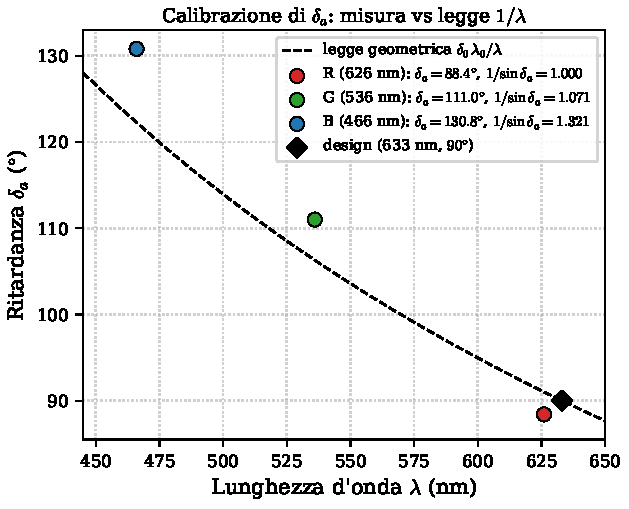
\includegraphics[width=0.62\textwidth]{Images/generated/lambdaquarti_50deg/s3_calibration.pdf}
    \caption{Calibrazione della ritardanza $\delta_a$ dell'analizzatore $\lambda/4$. I tre punti colorati sono i valori misurati direttamente dal dataset \texttt{lambdaquarti} in modo non circolare e indipendente dal materiale; la curva tratteggiata è la sola legge geometrica $\delta_0\,\lambda_0/\lambda$ di un ritardatore a singolo ordine, ancorata al punto di design (diamante nero, $\lambda_0 = \SI{633}{\nano\meter}$, $\delta_0 = 90^\circ$): \emph{non} un fit ai punti ma il riferimento minimo indipendente dal materiale. La misura la segue al rosso e cresce più ripidamente verso il blu, come atteso in presenza di dispersione normale della birifrangenza; la correzione $1/\sin\delta_a$ riportata in legenda cresce dal rosso, dove è prossima all'unità, al blu.}
    \label{fig:s3_calibration}
\end{figure}

L'adozione di questa correzione misurata, in luogo di quella calcolata da un tipico modello di dispersione di lamina a singolo ordine, sposta la ritardanza ricostruita dei campioni di non più di circa un grado, blu compreso, e lascia invariate le pendenze del nastro stratificato analizzato nella \cref{sec:risultati_nastro}. Questa insensibilità è essa stessa un risultato: la ricostruzione della ritardanza non dipende in modo critico dal modello di dispersione adottato per $S_3$, e l'obiezione di principio sulla scelta del materiale della lamina perde mordente sul piano quantitativo. Le sezioni seguenti applicano la correzione calibrata a campioni di ritardanza nota e crescente.

% ---------------------------------------------------------------------------
\section{Accuratezza della ricostruzione: lamine d'onda}
\label{sec:risultati_lamine}

\subsection{Lamina \texorpdfstring{$\lambda/4$}{lambda/4}}
\label{subsec:risultati_qw}

La lamina quarto d'onda ($\lambda_0 = \SI{633}{\nano\meter}$), orientata a circa \SI{50}{\degree}, è stata analizzata sui tre canali colore con la procedura comune a entrambe le lamine d'onda. Questo campione ha un ruolo speciale: è dello stesso tipo della lamina $\lambda/4$ impiegata come analizzatore di $S_3$, ed è dal suo dataset che si ricava la calibrazione non circolare della correzione cromatica di $S_3$ (\cref{sec:calibrazione_s3}). Analizzata qui come campione attraverso la pipeline completa, con la correzione già calibrata, ne riproduce per costruzione la ritardanza e ne documenta l'uniformità spaziale; il controllo di accuratezza genuino, il confronto fra ritardanza misurata e legge geometrica di singolo ordine senza assunzioni sul materiale, è quello discusso nella sezione di calibrazione.

La struttura del campione è visibile nelle mappe di intensità $S_0$ in \cref{fig:qw_s0}: il disco centrale corrisponde alla lamina a ritardanza uniforme, l'anello scuro alla montatura circolare che la sostiene, e lo sfondo libero alla luce diretta del display LCD, dove la ritardanza è prossima a zero.

\begin{figure}[H]
    \centering
    \subfloat[Canale R ($\lambda_\mathrm{eff} \approx \SI{626}{\nano\meter}$)]{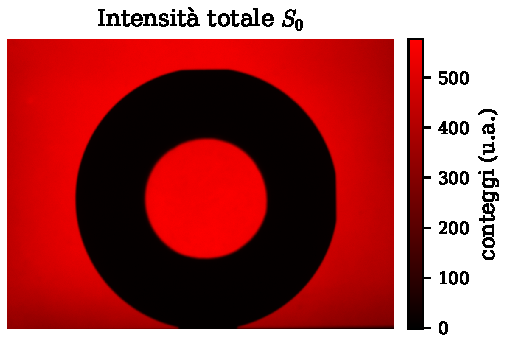
\includegraphics[height=0.205\textwidth]{Images/generated/lambdaquarti_50deg/R_S0.pdf}}\hfill
    \subfloat[Canale G ($\lambda_\mathrm{eff} \approx \SI{536}{\nano\meter}$)]{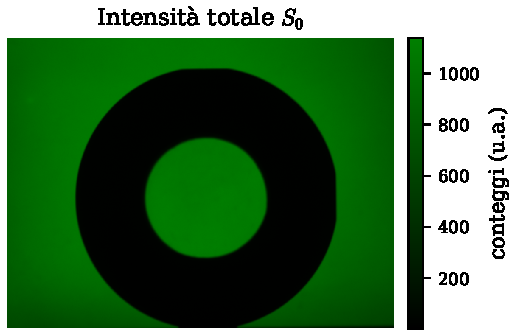
\includegraphics[height=0.205\textwidth]{Images/generated/lambdaquarti_50deg/G_S0.pdf}}\hfill
    \subfloat[Canale B ($\lambda_\mathrm{eff} \approx \SI{466}{\nano\meter}$)]{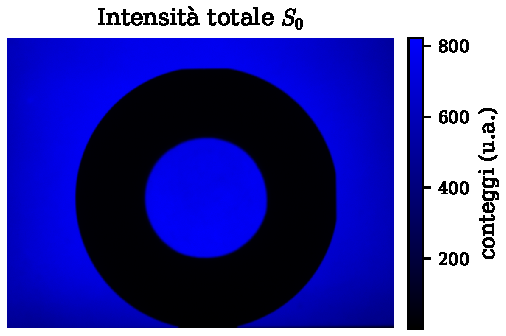
\includegraphics[height=0.205\textwidth]{Images/generated/lambdaquarti_50deg/B_S0.pdf}}
    \caption{Mappe di intensità $S_0$ per la lamina $\lambda/4$ sui tre canali del sensore. Il disco centrale corrisponde alla lamina, l'anello scuro alla montatura, lo sfondo all'illuminazione diretta del display LCD.}
    \label{fig:qw_s0}
\end{figure}

Le mappe dell'orientazione dell'asse veloce $\theta$ e della ritardanza $\delta$ sono riportate per i tre canali in \cref{fig:qw_theta_delta}. L'asse veloce è uniforme entro il disco della lamina, su un valore prossimo a $34^\circ$; lo scarto rispetto all'orientazione meccanica nominale di \SI{50}{\degree} corrisponde all'offset fra il riferimento del supporto della lamina e l'asse di polarizzazione incidente del display, rispetto al quale la pipeline misura tutti gli angoli polarimetrici (\cref{sec:allineamento}). La ritardanza è uniforme nello stesso disco e cresce dal canale rosso al canale blu, secondo la dispersione $\delta \propto 1/\lambda$ attesa per una lamina a singolo ordine. Le code di rumore aumentano verso il blu, dove il rapporto segnale-rumore di $S_3$ peggiora a causa della maggiore correzione cromatica applicata.

\begin{figure}[H]
    \centering
    \subfloat[$\theta$ , canale R]{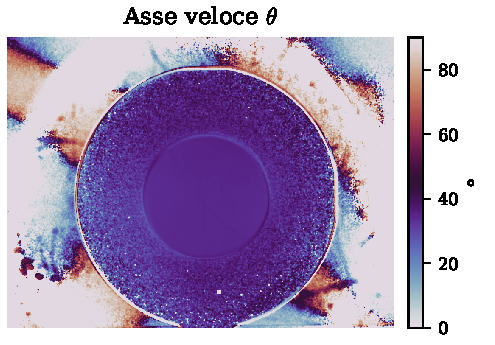
\includegraphics[height=0.205\textwidth]{Images/generated/lambdaquarti_50deg/R_theta.pdf}}\hfill
    \subfloat[$\theta$ , canale G]{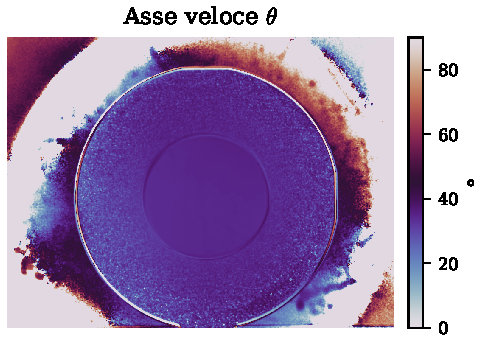
\includegraphics[height=0.205\textwidth]{Images/generated/lambdaquarti_50deg/G_theta.pdf}}\hfill
    \subfloat[$\theta$ , canale B]{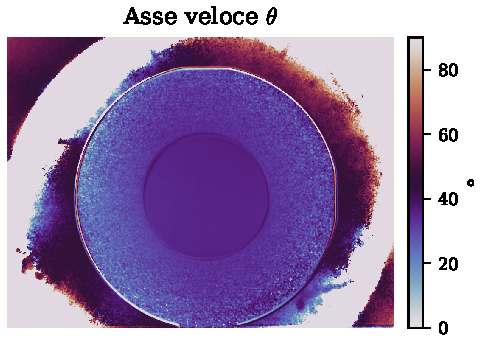
\includegraphics[height=0.205\textwidth]{Images/generated/lambdaquarti_50deg/B_theta.pdf}}\\
    \subfloat[$\delta$ , canale R]{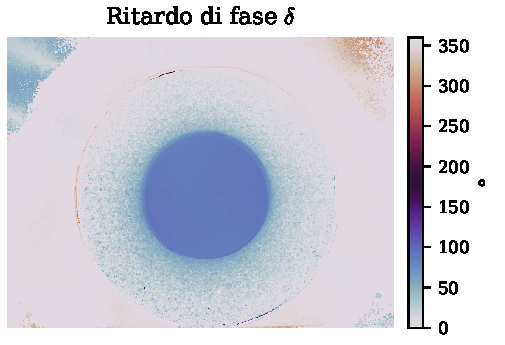
\includegraphics[height=0.205\textwidth]{Images/generated/lambdaquarti_50deg/R_delta.pdf}}\hfill
    \subfloat[$\delta$ , canale G]{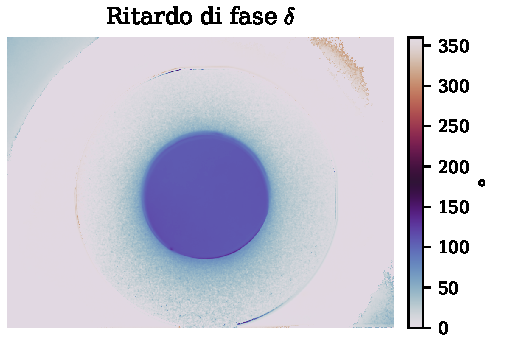
\includegraphics[height=0.205\textwidth]{Images/generated/lambdaquarti_50deg/G_delta.pdf}}\hfill
    \subfloat[$\delta$ , canale B]{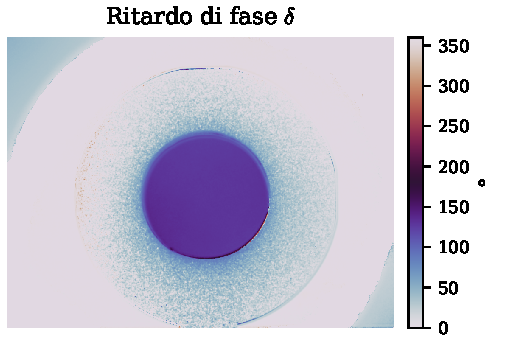
\includegraphics[height=0.205\textwidth]{Images/generated/lambdaquarti_50deg/B_delta.pdf}}
    \caption{Mappe dell'orientazione dell'asse veloce $\theta$ (riga superiore) e della ritardanza $\delta$ (riga inferiore) per la lamina $\lambda/4$, sui tre canali del sensore. L'asse veloce è uniforme entro il disco della lamina; la ritardanza cresce dal rosso al blu secondo la dispersione $\delta \propto 1/\lambda$ di una lamina a singolo ordine.}
    \label{fig:qw_theta_delta}
\end{figure}

La conversione della polarizzazione lineare in circolare, funzione caratteristica di una lamina quarto d'onda, è verificata direttamente dal modulo della componente circolare normalizzata nel disco. Per una lamina con asse veloce a $\theta$ e ritardanza $\delta_a$ il modello di propagazione (\cref{eq:s3_ritardatore}) prevede $|s_3| = \sin 2\theta \, \sin\delta_a \, p$, dove $p$ è il grado di polarizzazione locale: con $\theta \approx 34^\circ$ e i valori calibrati di $\delta_a$, l'atteso è $0{,}84$, $0{,}72$ e $0{,}57$ sui tre canali, contro valori misurati di $0{,}82$, $0{,}69$ e $0{,}54$, in accordo entro $0{,}03$. Il valore unitario del caso ideale, lamina a $45^\circ$ e luce completamente polarizzata, non viene raggiunto perché l'orientazione effettiva rispetto alla polarizzazione incidente è di circa $34^\circ$ e la lamina depolarizza parzialmente il fascio.

La stima quantitativa della ritardanza segue la stessa pipeline di clustering della \cref{sec:umap_clustering}: il cluster vincente HDBSCAN sull'embedding UMAP individua i pixel del disco della lamina e ne fornisce la mediana $\tilde\delta_{\mathrm{win}}$. Le tre stime per-canale, ottenute processando la lamina come campione con la correzione di $S_3$ calibrata, sono raccolte nella \cref{tab:qw_ritardanza} e confrontate con la legge geometrica di singolo ordine ancorata al design. La dispersione interna del cluster vincente, quantificata dalla deviazione mediana assoluta circolare, non supera $1{,}2^\circ$ su alcun canale: si tratta di un indicatore dell'omogeneità della regione selezionata, da non confondersi con l'accuratezza assoluta della misura (\cref{sec:discussione}). Esse coincidono per costruzione con la calibrazione (\cref{tab:s3_calibrazione}) a meno di una lieve differenza, più marcata al blu, dovuta al bias di depolarizzazione della lettura combinata coseno-seno della ritardanza, che tende a riavvicinare il valore a $90^\circ$. Le stime sono fittate con la legge di dispersione $\delta(\lambda) = k/\lambda$ di una lamina a singolo ordine; il punto di design $(\lambda_0 = \SI{633}{\nano\meter},\,\delta_0 = 90^\circ)$ è riportato come riferimento ma non incluso nel fit, condotto sui soli tre punti misurati. Il risultato è in \cref{fig:qw_delta_fit}.

\begin{table}[H]
    \centering
    \caption{Ritardanza della lamina $\lambda/4$ analizzata \emph{come campione} ($\lambda_0 = \SI{633}{\nano\meter}$), estratta dalla mediana del cluster vincente HDBSCAN sull'embedding UMAP e processata con la correzione di $S_3$ calibrata (\cref{sec:calibrazione_s3}), confrontata con la sola legge geometrica $\delta(\lambda) = 90^\circ \cdot \lambda_0/\lambda$ di un ritardatore a singolo ordine, indipendente dal materiale. Lo scarto, in eccesso crescente verso il blu, ingloba il contributo fisico della dispersione normale della birifrangenza, che si somma al fattore $1/\lambda$. La lieve differenza rispetto ai valori di calibrazione (\cref{tab:s3_calibrazione}), più marcata al blu, riflette il bias di depolarizzazione della lettura combinata coseno-seno della ritardanza.}
    \label{tab:qw_ritardanza}
    \begin{tabular}{lcccc}
        \hline
        \textbf{Canale} & $\lambda_\mathrm{eff}$ [\si{\nano\meter}] & $\tilde\delta_\mathrm{win}$ [\si{\degree}] & $\delta_\mathrm{geom}$ [\si{\degree}] & Scarto [\si{\degree}] \\
        \hline
        Rosso & 626 & $87{,}1$  & $91{,}0$  & $-3{,}9$ \\
        Verde & 536 & $108{,}6$ & $106{,}3$ & $+2{,}3$ \\
        Blu   & 466 & $128{,}5$ & $122{,}3$ & $+6{,}2$ \\
        \hline
    \end{tabular}
\end{table}

\begin{figure}[H]
    \centering
    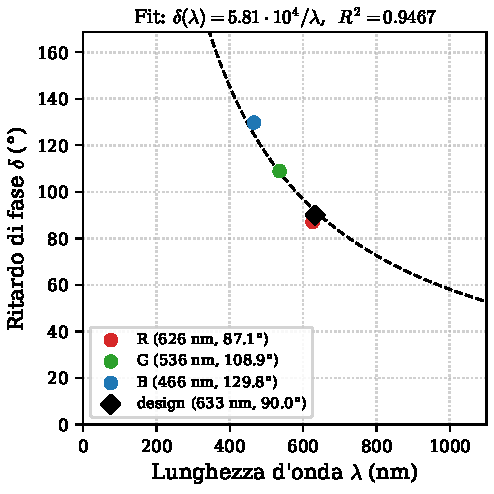
\includegraphics[width=0.55\textwidth]{Images/generated/lambdaquarti_50deg/delta_lambda_fit.pdf}
    \caption{Fit di dispersione $\delta(\lambda) = k/\lambda$ sulla lamina $\lambda/4$. I tre punti colorati sono le stime $\tilde\delta_{\mathrm{win}}$ del cluster vincente HDBSCAN per ciascun canale; il diamante nero è il punto di design $(\lambda_0 = \SI{633}{\nano\meter},\,\delta_0 = 90^\circ)$, riportato come riferimento e non incluso nel fit. La curva tratteggiata è il fit non lineare ai minimi quadrati sui soli tre punti misurati.}
    \label{fig:qw_delta_fit}
\end{figure}

\subsection{Lamina \texorpdfstring{$\lambda/2$}{lambda/2}}
\label{subsec:risultati_hw}

La lamina mezz'onda, di cui il costruttore dichiara la sola ritardanza nominale di mezz'onda alla lunghezza d'onda di design $\lambda_0 = \SI{633}{\nano\meter}$, orientata a circa \SI{50}{\degree}, è stata analizzata sui tre canali colore con l'obiettivo di validare la ricostruzione della ritardanza in un regime di forte dispersione cromatica, oltre la lunghezza d'onda di progetto; come si vedrà, la misura rivela un ritardatore con dispersione di ritardanza \emph{inversa}, della famiglia dei ritardatori a largo spettro, informazione non deducibile dall'etichetta. La struttura macroscopica del campione è visibile nelle mappe di intensità $S_0$ in \cref{fig:hw_s0}: si distingue il disco centrale della lamina, la montatura metallica circolare che la sostiene e lo sfondo libero illuminato dal display LCD. Il contrasto fra le tre acquisizioni RGB riflette unicamente la trasmissività spettrale del sistema sorgente-lamina-sensore e non dipende dallo stato di polarizzazione locale.

\begin{figure}[H]
    \centering
    \subfloat[Canale R ($\lambda_\mathrm{eff} \approx \SI{626}{\nano\meter}$)]{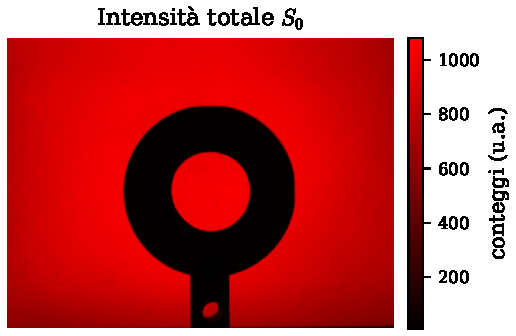
\includegraphics[height=0.205\textwidth]{Images/generated/lambdamezzi_50deg/R_S0.pdf}}\hfill
    \subfloat[Canale G ($\lambda_\mathrm{eff} \approx \SI{536}{\nano\meter}$)]{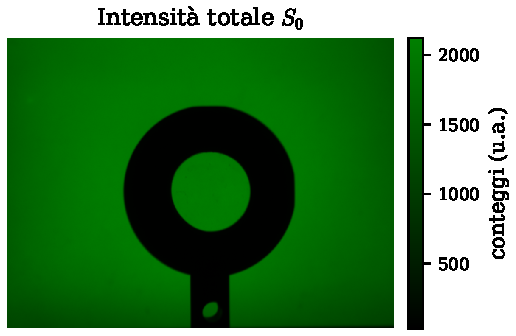
\includegraphics[height=0.205\textwidth]{Images/generated/lambdamezzi_50deg/G_S0.pdf}}\hfill
    \subfloat[Canale B ($\lambda_\mathrm{eff} \approx \SI{466}{\nano\meter}$)]{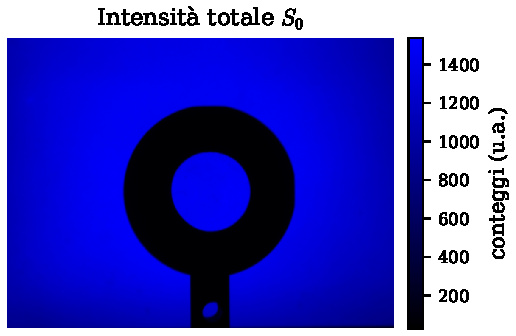
\includegraphics[height=0.205\textwidth]{Images/generated/lambdamezzi_50deg/B_S0.pdf}}
    \caption{Mappe di intensità $S_0$ per la lamina $\lambda/2$ sui tre canali del sensore. Il disco centrale corrisponde alla lamina, l'anello scuro alla montatura, lo sfondo all'illuminazione diretta del display LCD.}
    \label{fig:hw_s0}
\end{figure}

Le mappe dell'orientazione dell'asse veloce $\theta$ e della ritardanza $\delta$ sono riportate per i tre canali colore in \cref{fig:hw_theta_delta}. L'asse veloce risulta uniforme entro il disco della lamina, su un valore prossimo a $38^\circ$; lo scarto rispetto all'orientazione meccanica nominale di \SI{50}{\degree} corrisponde all'offset fra il riferimento del supporto della lamina e l'asse di polarizzazione incidente del display, rispetto al quale la pipeline misura tutti gli angoli polarimetrici (\cref{sec:allineamento}), e la differenza di qualche grado rispetto all'offset della lamina $\lambda/4$ (asse a circa $34^\circ$, \cref{subsec:risultati_qw}) rientra nella tolleranza dell'impostazione manuale dell'orientazione sul supporto. La ritardanza è anch'essa uniforme nel disco, ma il suo valore \emph{decresce} passando dal canale rosso al canale blu, in direzione opposta a quella attesa per una lamina a singolo ordine, in cui $\delta \propto 1/\lambda$ cresce verso le lunghezze d'onda corte. L'algoritmo di estrazione discusso nella \cref{subsec:modello_retardance} restituisce $\delta$ nell'intervallo $[0^\circ, 360^\circ)$ tramite $\arctan_2(\sin\delta, \cos\delta)$, con il segno di $\sin\delta$ fissato univocamente dal parametro $S_3$; il valore ricostruito è pertanto privo di ambiguità e questa decrescita è una caratteristica genuina del dato, la cui interpretazione è sviluppata più avanti.

\begin{figure}[H]
    \centering
    \subfloat[$\theta$ , canale R]{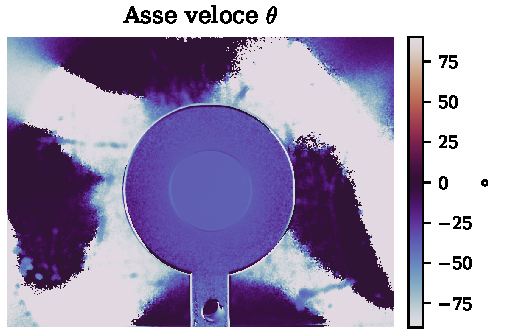
\includegraphics[height=0.205\textwidth]{Images/generated/lambdamezzi_50deg/R_theta.pdf}}\hfill
    \subfloat[$\theta$ , canale G]{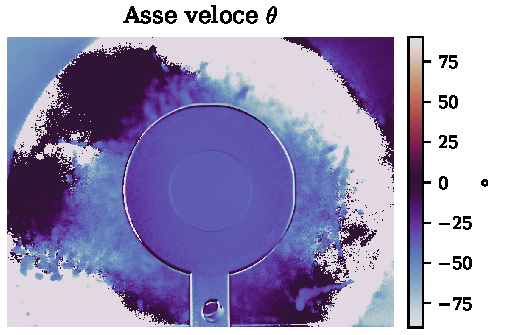
\includegraphics[height=0.205\textwidth]{Images/generated/lambdamezzi_50deg/G_theta.pdf}}\hfill
    \subfloat[$\theta$ , canale B]{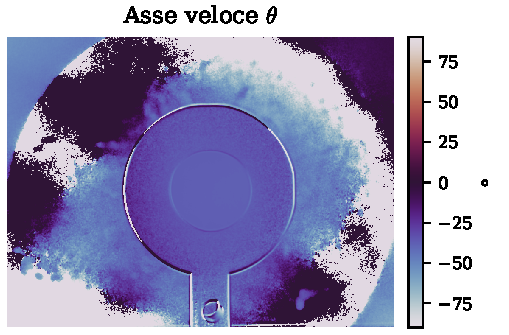
\includegraphics[height=0.205\textwidth]{Images/generated/lambdamezzi_50deg/B_theta.pdf}}\\
    \subfloat[$\delta$ , canale R]{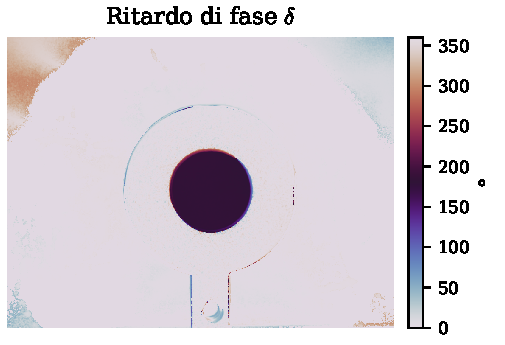
\includegraphics[height=0.205\textwidth]{Images/generated/lambdamezzi_50deg/R_delta.pdf}}\hfill
    \subfloat[$\delta$ , canale G]{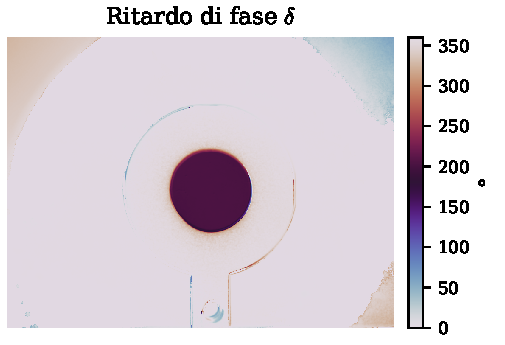
\includegraphics[height=0.205\textwidth]{Images/generated/lambdamezzi_50deg/G_delta.pdf}}\hfill
    \subfloat[$\delta$ , canale B]{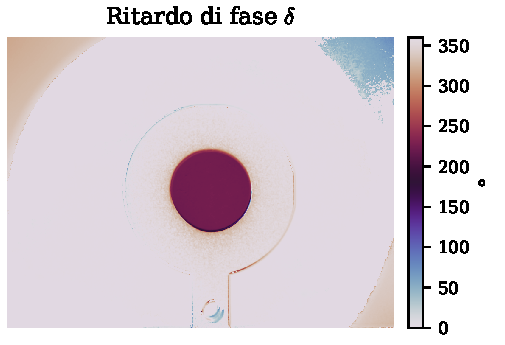
\includegraphics[height=0.205\textwidth]{Images/generated/lambdamezzi_50deg/B_delta.pdf}}
    \caption{Mappe dell'orientazione dell'asse veloce $\theta$ (riga superiore) e della ritardanza $\delta$ (riga inferiore) per la lamina $\lambda/2$, sui tre canali del sensore. L'asse veloce è uniforme entro il disco della lamina; la ritardanza, anch'essa uniforme, \emph{decresce} dal rosso al blu, in direzione opposta alla legge $\delta \propto 1/\lambda$ di un ritardatore a dispersione normale. Tale comportamento, dopo l'esclusione quantitativa delle spiegazioni alternative, è attribuito nel testo a una dispersione di ritardanza inversa (ritardatore a largo spettro). La \emph{colormap} ciclica \texttt{twilight} sull'intero giro $[0^\circ, 360^\circ)$ è impiegata per $\delta$.}
    \label{fig:hw_theta_delta}
\end{figure}

La funzione caratteristica di una lamina mezz'onda, la rotazione dell'azimut di polarizzazione di un angolo pari al doppio dell'orientazione dell'asse, è verificata sull'AoLP del disco. Al canale rosso, dove la ritardanza misurata di $\approx 177^\circ$ è prossima alla mezz'onda ideale, l'AoLP del cluster della lamina vale $+75{,}7^\circ$, in accordo entro un grado con il valore $2\theta \approx 76^\circ$ atteso per l'asse a $\theta \approx 38^\circ$; sui canali verde e blu l'AoLP scende progressivamente a $+72{,}8^\circ$ e $+70{,}4^\circ$, coerentemente con l'allontanamento della ritardanza dal valore di mezz'onda, che rende lo stato uscente ellittico e ne sposta l'azimut.

Per ottenere una stima quantitativa della ritardanza non condizionata da scelte soggettive della regione di interesse si è ricorsi alla pipeline di clustering descritta nella \cref{sec:umap_clustering}: il vettore di feature $(s_1, s_2, s_3, \mathrm{DoLP})$ viene proiettato in due dimensioni tramite UMAP e l'embedding viene segmentato con HDBSCAN. Il cluster di sfondo, che concentra la maggior parte della massa statistica, identifica la posizione angolare di riferimento sul cerchio di $\delta$; il cluster vincente, individuato dallo score $\mathcal{S}_k = f_k \cdot R_k \cdot (\Delta\delta_k)^2$, coincide con i pixel della lamina e fornisce direttamente la stima $\tilde\delta_{\mathrm{win}}$. La quadratura della distanza angolare penalizza i grandi cluster centrati sulla mediana globale, sterilizzando il rischio di selezionare lo sfondo come falso positivo. Le tre stime $\tilde\delta_R$, $\tilde\delta_G$, $\tilde\delta_B$ così ottenute alle rispettive lunghezze d'onda centroidi, con una deviazione mediana assoluta entro il cluster inferiore a $0{,}6^\circ$ su tutti i canali, sono raccolte nella \cref{tab:hw_ritardanza} e confrontate con la previsione $\delta(\lambda) = k/\lambda$ propria di una lamina a singolo ordine (\cref{eq:fit_dispersione} con $p=1$), normalizzata al punto di design $(\lambda_0 = \SI{633}{\nano\meter},\,\delta_0 = 180^\circ)$ dichiarato dal costruttore.

\begin{table}[H]
    \centering
    \caption{Ritardanza della lamina $\lambda/2$ estratta dalla mediana del cluster vincente HDBSCAN sull'embedding UMAP, confrontata con la previsione a singolo ordine $\delta_\mathrm{teorico} = \delta_0 \cdot \lambda_0/\lambda$ ($\delta_0 = 180^\circ$ alla lunghezza d'onda di design $\lambda_0 = \SI{633}{\nano\meter}$). Questa è la dipendenza minima attesa per un ritardatore a singolo passaggio in regime di dispersione normale, fissata dal solo fattore geometrico $1/\lambda$; la dispersione di birifrangenza, se normale, non farebbe che accentuarne la crescita verso il blu. La ritardanza misurata \emph{decresce} invece verso il blu, in direzione opposta alla previsione, che \emph{cresce}: la lamina non è riconducibile a un ritardatore a dispersione normale, e l'analisi nel testo esclude quantitativamente anche l'avvolgimento multi-ordine, attribuendo la decrescita a una dispersione di ritardanza inversa.}
    \label{tab:hw_ritardanza}
    \begin{tabular}{lcccc}
        \hline
        \textbf{Canale} & $\lambda_\mathrm{eff}$ [\si{\nano\meter}] & $\tilde\delta_\mathrm{win}$ [\si{\degree}] & $\delta_\mathrm{teorico}$ [\si{\degree}] & Scarto [\si{\degree}] \\
        \hline
        Rosso & 626 & $176{,}9$ & $182{,}0$ & $-5{,}1$ \\
        Verde & 536 & $156{,}8$ & $212{,}6$ & $-55{,}8$ \\
        Blu   & 466 & $134{,}5$ & $244{,}5$ & $-110{,}0$ \\
        \hline
    \end{tabular}
\end{table}

I tre valori misurati decrescono in modo monotono dal rosso al blu ($176{,}9 \to 156{,}8 \to 134{,}5^\circ$), in direzione opposta alla previsione a dispersione normale, che cresce ($182{,}0 \to 212{,}6 \to 244{,}5^\circ$). Per un ritardatore attraversato una sola volta vale $\delta = 2\pi\,\Delta n(\lambda)\,d/\lambda$, e in regime di dispersione normale entrambi i fattori spingono $\delta$ verso l'alto alle lunghezze d'onda corte. Conviene riformulare il dato in termini di ritardo ottico $\mathrm{Re} = \delta\,\lambda/360^\circ = \Delta n\, d$, la grandezza propria del materiale, depurata dal fattore geometrico: la misura corrisponde a $\mathrm{Re} = 308 \to 233 \to 174$~nm dal rosso al blu. Su una lamina priva di marcature, peraltro, l'assegnazione di quale asse sia il veloce è intrinsecamente ambigua, e l'assegnazione complementare ($\delta \to 360^\circ - \delta$, ovvero $183{,}1/203{,}2/225{,}5^\circ$) fornisce $\mathrm{Re} = 318 \to 303 \to 292$~nm: il ritardo ottico decresce verso il blu in entrambi i casi, del $43\%$ o dell'$8\%$ rispettivamente, sicché la conclusione qualitativa non dipende dall'ambiguità. Un fit empirico $\delta = k/\lambda^{\,n}$ restituisce $n \approx -0{,}9$ sul ramo misurato e $n \approx +0{,}7$ sul complementare: in entrambi i casi $|n| < 1$, mentre la dispersione normale impone $n \geq 1$.

Prima di interpretare il dato si sono vagliate le spiegazioni più economiche. Un errore sistematico della catena di analisi è escluso dal riscontro della lamina $\lambda/4$ (\cref{sec:calibrazione_s3}), che con lo stesso modello di Stokes, la stessa correzione cromatica di $S_3$ e le stesse lunghezze d'onda effettive cresce verso il blu come atteso. Un'inversione prodotta da assi veloce e lento scambiati è già contenuta nell'ambiguità di assegnazione discussa sopra e non cambia il verso del ritardo ottico; il modulo della componente circolare normalizzata fornisce in ogni caso un controllo indipendente da qualunque convenzione di segno: $|s_3|$ misurato nel disco vale $0{,}05/0{,}31/0{,}53$ sui tre canali, in accordo entro $0{,}02$ con il modello $p \sin 2\theta\, |\sin\delta|$ valutato sui valori misurati, mentre la dispersione normale ($\delta = 213/246^\circ$ a G/B) predirebbe $0{,}44/0{,}70$, incompatibile. Una depolarizzazione differenziale del campione è infine esclusa dal grado di polarizzazione, identico fra le due lamine a ciascun canale.

L'ipotesi a prima vista più naturale resta allora l'avvolgimento: una lamina \emph{multi-ordine}, la cui ritardanza vera supera più giri di $360^\circ$, campionata su tre sole bande spettrali, può mostrare valori avvolti che procedono all'indietro per sotto-campionamento, in analogia con l'effetto stroboscopico per cui una ruota in rapida rotazione appare girare al contrario in una ripresa a basso numero di fotogrammi. Questa interpretazione, in apparenza la più semplice, è però falsificabile con i dati a disposizione, perché i canali del sensore non sono monocromatici. Su una banda di larghezza finita la ritardanza vera di un multi-ordine varia di molte decine o centinaia di gradi, e la sovrapposizione incoerente degli stati uscenti depolarizza il segnale: la frazione di polarizzazione conservata dalla media di banda è
\begin{equation}
    |V| = \frac{\left|\int I(\lambda)\, e^{i\,\delta(\lambda)}\, d\lambda\right|}{\int I(\lambda)\, d\lambda},
    \label{eq:band_retention}
\end{equation}
dove $I(\lambda)$ è lo spettro efficace del canale. Valutata sugli spettri efficaci misurati (banda verde di larghezza $\approx \SI{40}{\nano\meter}$), la \cref{eq:band_retention} prevede per il canale verde $|V| \leq 0{,}74$ già all'ordine $2$ e $|V| \leq 0{,}4$ all'ordine $5$, cui corrisponde un grado di polarizzazione complessivo inferiore a $0{,}78$ e $0{,}5$ rispettivamente. Il valore misurato all'interno del disco è $0{,}85$, indistinguibile da quello della lamina $\lambda/4$ ($0{,}83$), che opera a ordine zero: l'avvolgimento multi-ordine è escluso, per qualunque scelta ragionevole del modello di banda. Lo stesso argomento, applicato alla $\lambda/4$, ne conferma a posteriori l'ordine zero.

Escluse le alternative, la decrescita è una proprietà reale del componente: la lamina è un ritardatore a basso ordine la cui dispersione di ritardanza è \emph{inversa}, con $\mathrm{Re}$ decrescente verso le lunghezze d'onda corte. Per un materiale naturale in regime di trasparenza questo comportamento sarebbe sorprendente, ed è per questo che l'ipotesi appare a prima vista più ardita dell'avvolgimento; per i film ritardatori, tuttavia, si tratta di una classe di prodotto consolidata. I ritardatori a largo spettro (acromatici) sono progettati proprio con $\mathrm{Re} \propto \lambda$, affinché $\delta$ resti costante sull'intero visibile, e si realizzano sia con copolimeri a dispersione di birifrangenza controllata~\cite{Uchiyama2012Copolycarbonate}, sia, al livello più economico, con film cellulosici, nei quali la dispersione inversa è una proprietà naturale del materiale: il comune cellophane è documentato in letteratura proprio come lamina a mezz'onda a largo spettro sull'intero visibile~\cite{OrtizGutierrez2001Cellophane}. Il dato quantitativo è coerente con questa famiglia: il rapporto di dispersione misurato $\mathrm{Re}(466)/\mathrm{Re}(536)$ vale $0{,}75$ sul ramo misurato e $0{,}96$ sul complementare, a cavallo del valore $466/536 = 0{,}87$ di un ritardatore piatto ideale. Al canale rosso, prossimo alla lunghezza d'onda di progetto, la lamina è effettivamente una mezz'onda ($\delta \approx 177^\circ$); in prossimità di $180^\circ$ la componente $S_3 \propto \sin\delta$ si annulla e $\delta$ è massimamente sensibile al rumore, sicché lo scarto di pochi gradi dal nominale non è significativo.

% DA RIVEDERE MANUALMENTE (ipotesi costruttiva riscritta 2026-06-12 dopo l'esclusione del multi-ordine; percorso completo in python/WAVEPLATE_INVESTIGATION.md)
La caratterizzazione congiunta delle due lamine suggerisce infine un'ipotesi costruttiva unitaria, avanzata come interpretazione plausibile e non come conclusione. Il ritardo ottico in gioco è di poche centinaia di nanometri ($\mathrm{Re}(633) \approx \SI{316}{\nano\meter}$ per la $\lambda/2$, $\approx \SI{158}{\nano\meter}$ per la $\lambda/4$): con le birifrangenze tipiche dei film polimerici e cellulosici ($\Delta n \approx 0{,}005$--$0{,}01$) bastano poche decine di micrometri di film, e lo spessore millimetrico osservato dei dischi è da attribuire a un substrato di vetro. Un film birifrangente sottile laminato fra due finestre di vetro è del resto la costruzione standard delle lamine polimeriche commerciali di fascia economica, proposte a catalogo come alternativa zero-order al quarzo. In questo quadro la $\lambda/4$ sarebbe ritagliata da un film a dispersione normale e la $\lambda/2$ da un film a dispersione inversa di tipo cellulosico o equivalente; per l'impiego didattico con sorgenti a banda larga una mezz'onda a largo spettro è peraltro funzionalmente preferibile a una monocromatica. Tre osservabili sostengono l'ipotesi: l'ordine zero di entrambe le lamine, la depolarizzazione residua identica fra le due (firma di una diffusione interna della stessa famiglia di materiali, non di un effetto di banda), e l'asse veloce che non ruota fra i canali colore (entro un grado), come si addice a un film monolitico e non a una pila di lamine sfalsate. Con due soli esemplari e tre bande spettrali larghe il materiale specifico non è identificabile e l'ipotesi resta indimostrabile; il suo merito è rendere conto in un quadro unico di ritardo, dispersione, spessore, depolarizzazione e costo. La calibrazione di $S_3$ non dipende in alcun modo da questa interpretazione, essendo fondata sulla misura diretta di $\delta_a$.

% ---------------------------------------------------------------------------
\section{Linearità e risoluzione spaziale: nastro adesivo}
\label{sec:risultati_nastro}

Le lamine d'onda, con ritardanza uniforme e nota, hanno confermato l'accuratezza puntuale della ricostruzione. Il campione seguente è stato scelto per verificare una proprietà diversa: la capacità del sistema di distinguere regioni con ritardanza crescente e di mantenere la linearità della risposta.

\subsection{Nastro adesivo stratificato}
\label{subsec:nastro_adesivo}

Il campione consiste in un vetrino con strati sovrapposti di nastro adesivo polimerico in configurazione simmetrica a gradino $1$-$2$-$3$-$4$-$5$-$4$-$3$-$2$-$1$, dove il numero indica gli strati attraversati dalla luce in ciascuna regione. A differenza delle lamine d'onda, la ritardanza non è qui uniforme ma cresce a gradini discreti con il numero di strati, e già il primo strato introduce un ritardo prossimo a $\SI{240}{\degree}$ al rosso: l'accumulo su cinque strati supera abbondantemente il giro completo, e la ritardanza misurata nell'intervallo $[0^\circ, 360^\circ)$ avvolge più volte. Il campione mette quindi alla prova due capacità distinte del sistema: la risoluzione spaziale necessaria a separare regioni adiacenti a diverso spessore, e la possibilità di ricostruire una risposta lineare nonostante l'avvolgimento modulo $360^\circ$. La simmetria della pila fornisce un controllo interno: regioni omologhe a sinistra e a destra del centro devono restituire la stessa ritardanza.

\begin{figure}[H]
    \centering
    \subfloat[Canale R ($\lambda_\mathrm{eff} \approx \SI{626}{\nano\meter}$)]{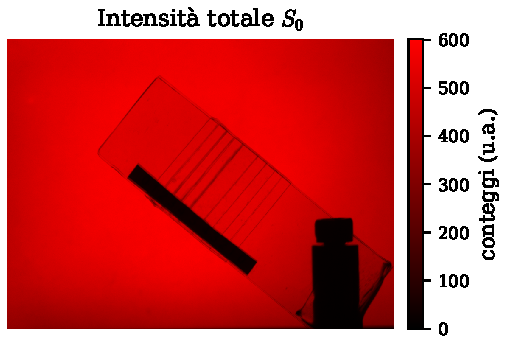
\includegraphics[height=0.205\textwidth]{Images/generated/strati_v2/R_S0.pdf}}\hfill
    \subfloat[Canale G ($\lambda_\mathrm{eff} \approx \SI{536}{\nano\meter}$)]{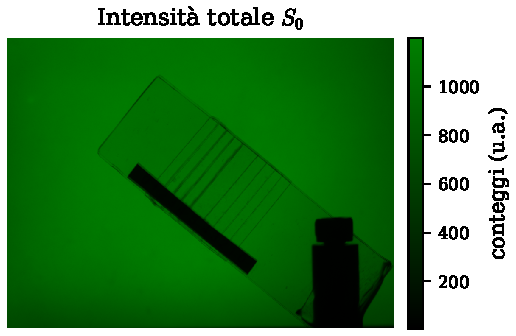
\includegraphics[height=0.205\textwidth]{Images/generated/strati_v2/G_S0.pdf}}\hfill
    \subfloat[Canale B ($\lambda_\mathrm{eff} \approx \SI{466}{\nano\meter}$)]{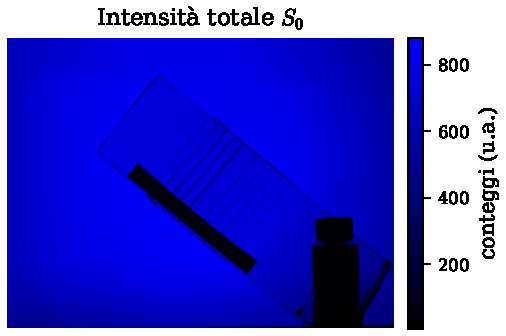
\includegraphics[height=0.205\textwidth]{Images/generated/strati_v2/B_S0.pdf}}
    \caption{Mappe di intensità $S_0$ del nastro adesivo stratificato sui tre canali del sensore. I gradini di spessore della pila simmetrica $1$-$2$-$3$-$4$-$5$-$4$-$3$-$2$-$1$ sono distinguibili come bande a diversa trasmissività.}
    \label{fig:nastro_s0}
\end{figure}

La mappa di ritardanza riflette direttamente la struttura a gradini, ma il valore letto in ciascuna banda è il residuo $\delta_\mathrm{vero} \bmod 360^\circ$: con un ritardo per strato prossimo a $\SI{240}{\degree}$, la successione dei valori misurati al crescere del numero di strati non è monotòna ma salta all'interno dell'intervallo $[0^\circ, 360^\circ)$ a ogni superamento del giro. L'istogramma della ritardanza sul campione presenta perciò un insieme discreto di picchi, uno per ciascun valore avvolto distinto, e la lettura strato per strato non è ricavabile dalla sola mappa. Per recuperare la ritardanza accumulata si ricorre all'analisi lungo una slice diagonale descritta nella \cref{sec:slice_dispersione}: una banda rettilinea spessa, orientata lungo la direzione di crescita della pila, viene campionata mediando circolarmente la ritardanza sulla larghezza, i plateau corrispondenti ai singoli strati vengono individuati per soglia sul gradiente ed etichettati da \texttt{1L} a \texttt{5} fino a \texttt{1R}, e un \emph{unwrap} cumulativo separato sul lato sinistro e destro ricostruisce la ritardanza vera prima dell'avvolgimento. Su questa si esegue il fit lineare attraverso l'origine $\delta = m\,n$.

Il canale rosso è il riferimento. La slice individua i nove plateau attesi (\cref{fig:nastro_slice_r}), con mediane che avvolgono da $\SI{247.6}{\degree}$ del primo strato fino a riavvolgersi più volte; l'istogramma in \cref{fig:nastro_hist_r} mostra la corrispondente struttura discreta dei valori avvolti sul campione. Dopo l'unwrap, i punti $(n, \delta)$ giacciono su una retta con pendenza $m_R = (240{,}2 \pm 0{,}9)~\si{\degree}$/strato (errore standard statistico del fit), coefficiente di determinazione $R^2 = 0{,}9994$ e scarto quadratico medio di $\SI{7.7}{\degree}$.

\begin{figure}[H]
    \centering
    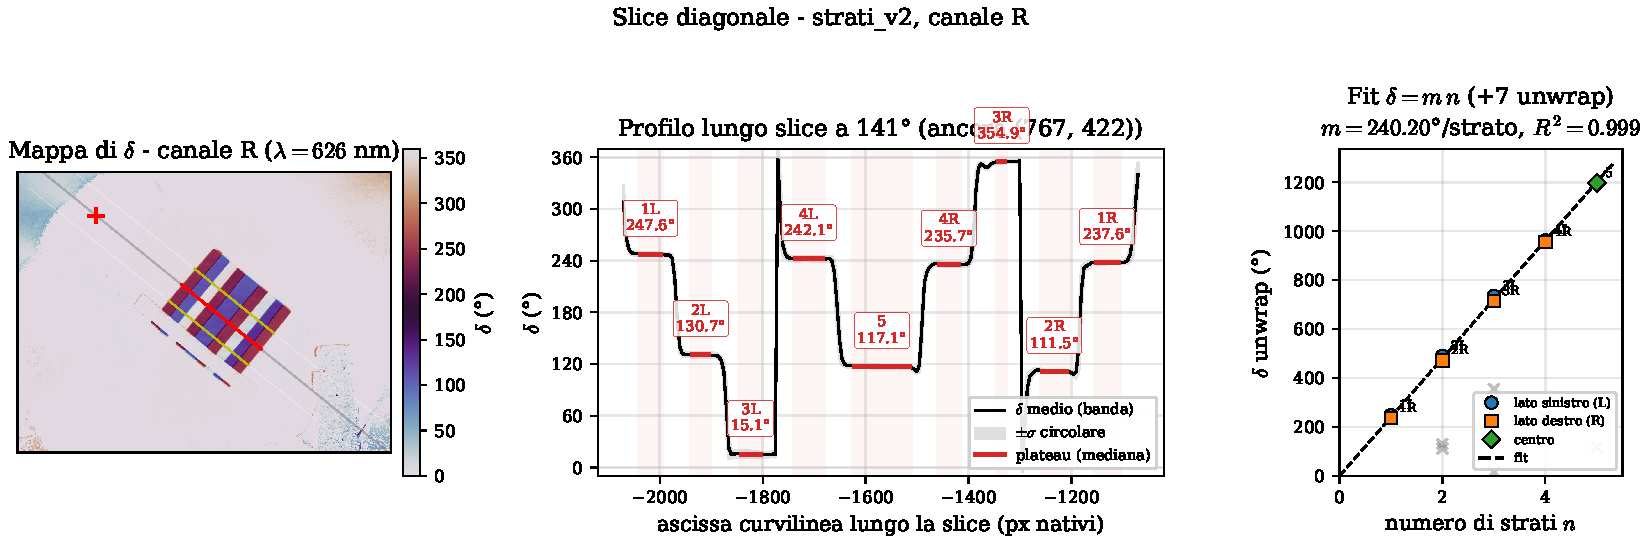
\includegraphics[width=\textwidth]{Images/generated/strati_v2/R_slice.pdf}
    \caption{Analisi della slice diagonale sul canale rosso. A sinistra la mappa di $\delta$ con la traccia della slice; al centro il profilo della ritardanza media lungo la slice con i plateau dei singoli strati evidenziati; a destra il fit lineare attraverso l'origine $\delta = m\,n$ dopo l'\emph{unwrap} cumulativo per lato.}
    \label{fig:nastro_slice_r}
\end{figure}

\begin{figure}[H]
    \centering
    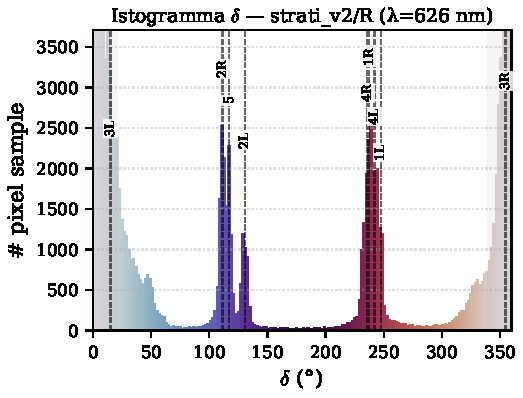
\includegraphics[width=0.62\textwidth]{Images/generated/strati_v2/R_hist_delta.pdf}
    \caption{Istogramma della ritardanza $\delta$ sul campione di nastro, canale rosso. Le linee verticali marcano le mediane dei plateau della slice, etichettate per strato; la distribuzione discreta riflette l'avvolgimento modulo $360^\circ$.}
    \label{fig:nastro_hist_r}
\end{figure}

Il canale verde (\cref{fig:nastro_slice_g,fig:nastro_hist_g}) ripete la procedura con un ritardo per strato maggiore, $m_G = (280{,}8 \pm 1{,}5)~\si{\degree}$/strato ($R^2 = 0{,}9988$, rms $\SI{12.9}{\degree}$), coerente con l'aumento atteso della ritardanza al diminuire della lunghezza d'onda.

\begin{figure}[H]
    \centering
    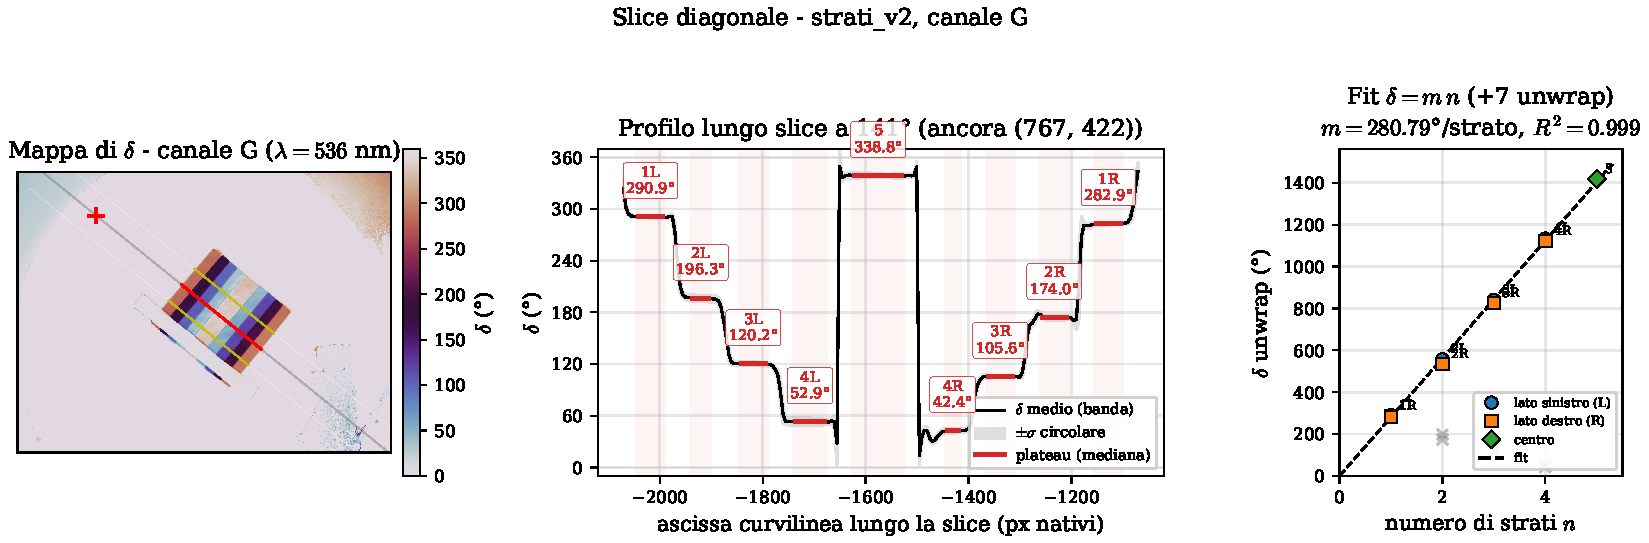
\includegraphics[width=\textwidth]{Images/generated/strati_v2/G_slice.pdf}
    \caption{Analisi della slice diagonale sul canale verde, con la stessa struttura a tre pannelli della \cref{fig:nastro_slice_r}.}
    \label{fig:nastro_slice_g}
\end{figure}

\begin{figure}[H]
    \centering
    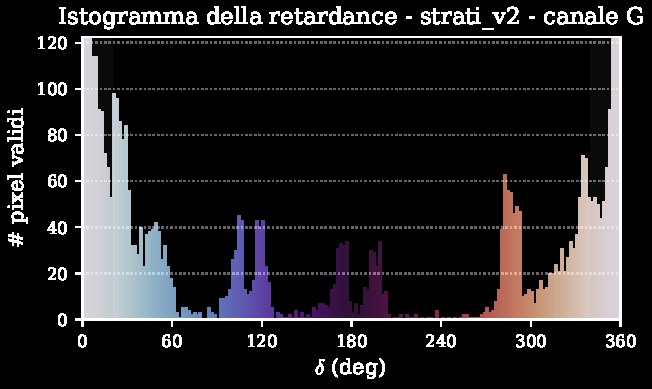
\includegraphics[width=0.62\textwidth]{Images/generated/strati_v2/G_hist_delta.pdf}
    \caption{Istogramma della ritardanza $\delta$ sul campione di nastro, canale verde, con le mediane dei plateau della slice.}
    \label{fig:nastro_hist_g}
\end{figure}

Il canale blu (\cref{fig:nastro_slice_b,fig:nastro_hist_b}) presenta il ritardo per strato più elevato, $m_B = (316{,}8 \pm 1{,}7)~\si{\degree}$/strato ($R^2 = 0{,}9987$, rms $\SI{14.8}{\degree}$); lo scarto quadratico medio cresce dal rosso al blu di pari passo con il peggioramento del rapporto segnale-rumore alle lunghezze d'onda corte.

\begin{figure}[H]
    \centering
    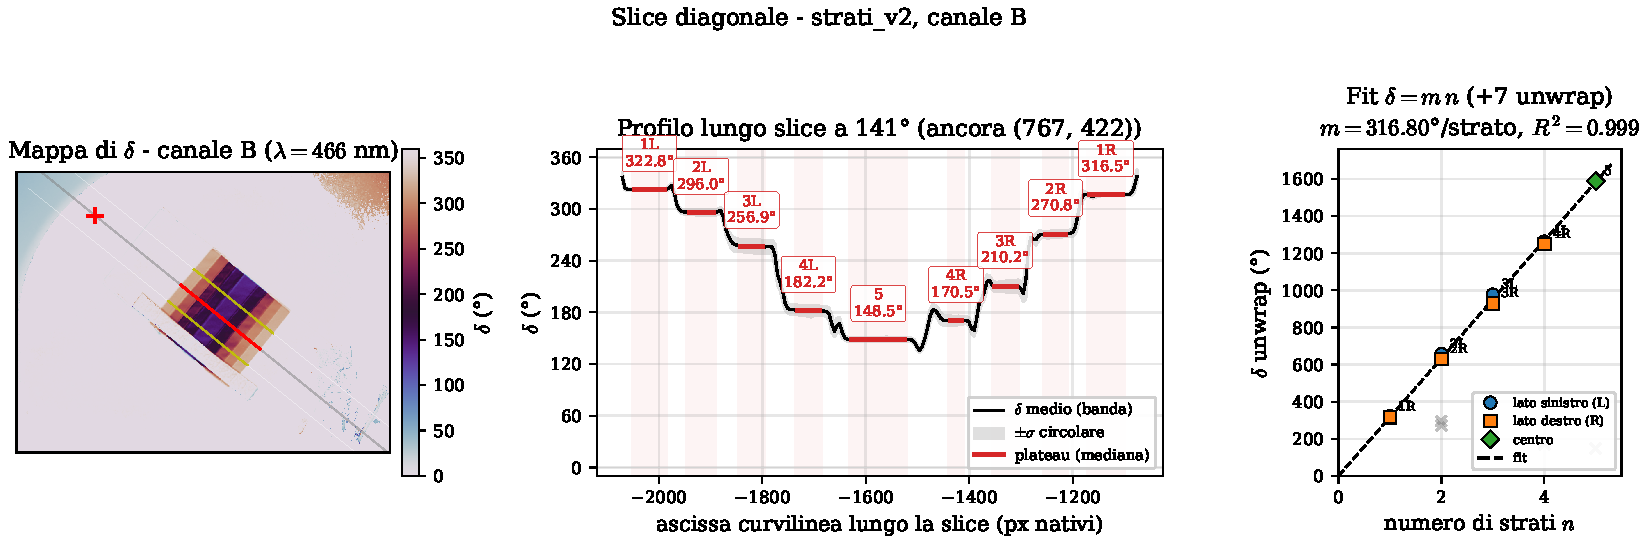
\includegraphics[width=\textwidth]{Images/generated/strati_v2/B_slice.pdf}
    \caption{Analisi della slice diagonale sul canale blu, con la stessa struttura a tre pannelli della \cref{fig:nastro_slice_r}.}
    \label{fig:nastro_slice_b}
\end{figure}

\begin{figure}[H]
    \centering
    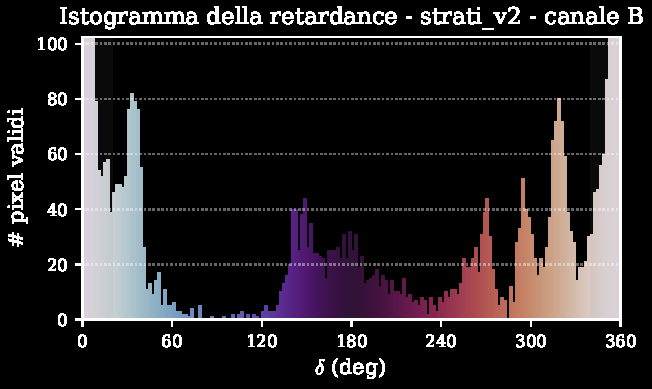
\includegraphics[width=0.62\textwidth]{Images/generated/strati_v2/B_hist_delta.pdf}
    \caption{Istogramma della ritardanza $\delta$ sul campione di nastro, canale blu, con le mediane dei plateau della slice.}
    \label{fig:nastro_hist_b}
\end{figure}

La \cref{tab:nastro_plateau} raccoglie le mediane di ritardanza dei nove plateau, così come misurate (avvolte in $[0^\circ, 360^\circ)$), per i tre canali; la non-monotonia delle colonne è la manifestazione diretta dell'avvolgimento. La \cref{tab:nastro_slope} riassume invece le pendenze ricavate dal fit lineare dopo l'unwrap.

\begin{table}[H]
    \centering
    \caption{Mediana della ritardanza $\delta$ misurata (avvolta in $[0^\circ, 360^\circ)$) per ciascun plateau della slice, sui tre canali. Le etichette indicano il numero di strati e il lato (L sinistro, R destro) rispetto al centro della pila.}
    \label{tab:nastro_plateau}
    \begin{tabular}{lccccccccc}
        \hline
        \textbf{Canale} & 1L & 2L & 3L & 4L & 5 & 4R & 3R & 2R & 1R \\
        \hline
        Rosso & $247{,}6$ & $130{,}7$ & $15{,}1$  & $242{,}1$ & $117{,}1$ & $235{,}7$ & $354{,}9$ & $111{,}5$ & $237{,}6$ \\
        Verde & $290{,}6$ & $196{,}6$ & $119{,}8$ & $53{,}5$  & $338{,}5$ & $42{,}9$  & $105{,}4$ & $173{,}9$ & $282{,}7$ \\
        Blu   & $321{,}2$ & $295{,}3$ & $258{,}5$ & $182{,}3$ & $147{,}2$ & $169{,}9$ & $212{,}1$ & $271{,}9$ & $315{,}2$ \\
        \hline
    \end{tabular}
\end{table}

\begin{table}[H]
    \centering
    \caption{Ritardo di fase per singolo strato di nastro adesivo, ricavato dal fit lineare attraverso l'origine $\delta = m\,n$ sui plateau della slice dopo \emph{unwrap}. L'incertezza su $m$ è l'errore standard statistico del fit sui nove plateau, ricavato dai residui; non include i contributi sistematici discussi nella \cref{sec:discussione}.}
    \label{tab:nastro_slope}
    \begin{tabular}{lcccc}
        \hline
        \textbf{Canale} & $\lambda_\mathrm{eff}$ [\si{\nano\meter}] & $m$ [\si{\degree}/strato] & $R^2$ & rms [\si{\degree}] \\
        \hline
        Rosso & 626 & $240{,}2 \pm 0{,}9$ & $0{,}9994$ & $7{,}7$  \\
        Verde & 536 & $280{,}8 \pm 1{,}5$ & $0{,}9988$ & $12{,}9$ \\
        Blu   & 466 & $316{,}8 \pm 1{,}7$ & $0{,}9987$ & $14{,}8$ \\
        \hline
    \end{tabular}
\end{table}

La linearità della risposta è eccellente su tutti e tre i canali, con $R^2 > 0{,}998$: il sistema ricostruisce una ritardanza accumulata fino a oltre $\SI{1500}{\degree}$ mantenendo la proporzionalità diretta con il numero di strati, una volta risolto l'avvolgimento tramite l'unwrap geometrico della slice. La simmetria della pila è rispettata entro pochi gradi sulla maggior parte dei plateau, confermando la coerenza spaziale della ricostruzione.

Il confronto delle regioni omologhe a tre strati evidenzia un'asimmetria residua fra lato sinistro e destro: contenuta sul rosso ($\SI{735.1}{\degree}$ contro $\SI{714.9}{\degree}$, $\SI{20.2}{\degree}$) e sul verde ($\SI{839.8}{\degree}$ contro $\SI{825.4}{\degree}$, $\SI{14.3}{\degree}$), essa sale a $\SI{46.4}{\degree}$ sul blu ($\SI{978.5}{\degree}$ contro $\SI{932.1}{\degree}$). L'effetto è confinato al terzo strato e al solo canale blu, non comparendo negli altri strati né sugli altri canali, ed è quindi incompatibile con un'asimmetria fisica generica del campione. Le verifiche condotte hanno escluso difetti di allineamento dei frame, depolarizzazione locale e asimmetrie nella distribuzione dei vettori di Stokes; la causa, plausibilmente una registrazione cromatica imperfetta del canale blu o un'interferenza sottile selettiva negli strati di adesivo, resta non identificata. Trattandosi di un'anomalia localizzata a un singolo punto, essa non influisce né sulla pendenza media né sulla linearità della risposta ($R^2 > 0{,}998$), entrambe ricavate dal fit complessivo sui nove plateau.

La dipendenza della ritardanza per strato dalla lunghezza d'onda è riassunta dai due grafici di \cref{fig:nastro_fit}. Il primo riporta i valori srotolati di $\delta$ in funzione del numero di strati per i tre canali, con le rispettive rette di fit attraverso l'origine; il secondo riporta le tre pendenze $m_c$ in funzione della lunghezza d'onda, con il fit di dispersione $m(\lambda) = k/\lambda$. Il fit restituisce $k = (1{,}492 \pm 0{,}010)\cdot10^{5}~\si{\degree\nano\meter}$/strato con $R^2 = 0{,}993$, dove l'incertezza è l'errore standard statistico del fit. Il rapporto fra le pendenze agli estremi spettrali, $m_B/m_R = 316{,}8/240{,}2 = 1{,}319$, è leggermente inferiore al rapporto puramente geometrico $\lambda_R/\lambda_B = 626/466 = 1{,}343$. La decomposizione per canale chiarisce la natura dello scarto: il prodotto $m \cdot \lambda$, costante per una dispersione puramente geometrica, coincide fra rosso e verde entro lo $0{,}1\%$, mentre il blu risulta inferiore dell'$1{,}8\%$. Una dispersione normale della birifrangenza, con $\Delta n$ crescente verso il blu come atteso per un polimero stirato, sposterebbe il rapporto nella direzione opposta; lo scarto, di segno contrario e confinato al solo canale blu, è dunque da attribuire a un residuo sistematico di quel canale, lo stesso interessato dall'anomalia locale discussa sopra, piuttosto che a una proprietà del materiale. L'effetto, dell'ordine del punto percentuale, non incide sulla linearità della risposta.

\begin{figure}[H]
    \centering
    \subfloat[Ritardanza srotolata in funzione del numero di strati, tre canali, con fit lineare attraverso l'origine.]{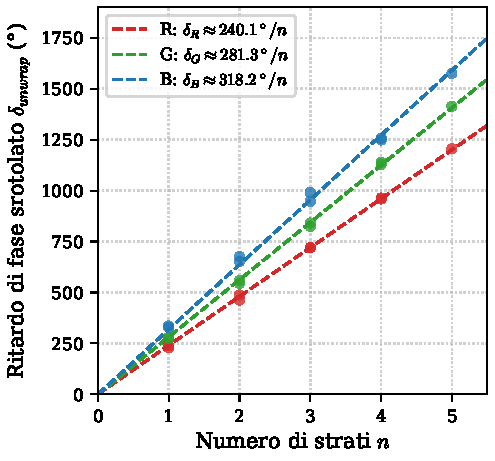
\includegraphics[width=0.46\textwidth]{Images/generated/strati_fit/fit_strati_linear.pdf}}\hfill
    \subfloat[Pendenza per strato in funzione della lunghezza d'onda, con fit di dispersione $m(\lambda) = k/\lambda$.]{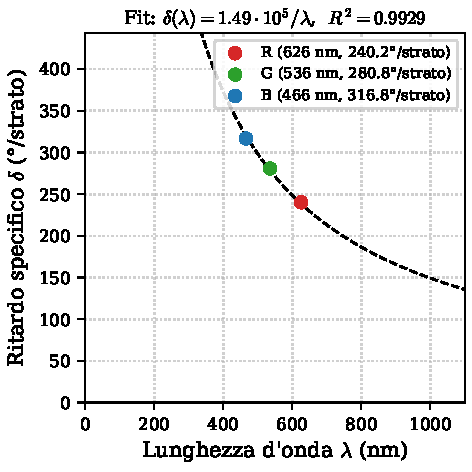
\includegraphics[width=0.46\textwidth]{Images/generated/strati_fit/fit_lambda_inverse.pdf}}
    \caption{Dipendenza spettrale della ritardanza del nastro adesivo. A sinistra la linearità $\delta = m\,n$ sui tre canali; a destra la dispersione delle pendenze, ben descritta dalla legge $m \propto 1/\lambda$ propria di un materiale a birifrangenza debolmente dispersiva.}
    \label{fig:nastro_fit}
\end{figure}

% ---------------------------------------------------------------------------
\section{Versatilità del sistema}
\label{sec:risultati_versatilita}

Dopo aver verificato che il polarimetro produce mappe coerenti per campioni birifrangenti, si passa a fenomeni fisicamente distinti per dimostrare la generalità del metodo.

\subsection{Soluzione di saccarosio}
\label{subsec:soluzione_zucchero}

La soluzione di saccarosio in acqua è otticamente attiva: il saccarosio destrogiro ruota il piano di polarizzazione della luce trasmessa di un angolo proporzionale al cammino ottico e alla concentrazione. A differenza della birifrangenza, l'attività ottica agisce sulle sole componenti lineari $S_1$ e $S_2$ senza coinvolgere $S_3$, e si manifesta come una rotazione rigida e spazialmente uniforme dell'angolo di polarizzazione lineare. La soluzione è contenuta in una boccetta a facce piane parallele di spessore interno $L = \SI{13}{\milli\meter}$; lo sfondo libero, allineato a $\mathrm{AoLP} \approx \SI{0}{\degree}$ per costruzione (\cref{sec:allineamento}), fornisce il riferimento rispetto al quale si misura la rotazione. Nella convenzione adottata (\cref{subsec:stokes_def}) una rotazione destrogira corrisponde a un AoLP negativo: la misura restituisce infatti un AoLP del cluster della soluzione sistematicamente negativo, da $-3{,}95^\circ$ al rosso a $-6{,}12^\circ$ al blu, in accordo con il carattere destrogiro del saccarosio e come conferma sperimentale indipendente della convenzione di segno. Nel seguito si indica con $\psi = |\mathrm{AoLP}|$ il modulo di tale rotazione, impiegato nella legge di Biot con il potere rotatorio specifico tabulato $[\alpha] > 0$ (convenzione chimica per le sostanze destrogire).

\begin{figure}[H]
    \centering
    \subfloat[Canale R ($\lambda_\mathrm{eff} \approx \SI{626}{\nano\meter}$)]{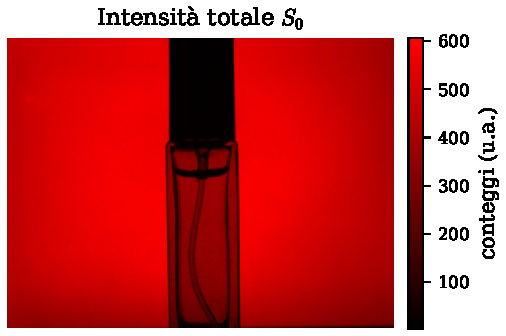
\includegraphics[height=0.205\textwidth]{Images/generated/zucchero/R_S0.pdf}}\hfill
    \subfloat[Canale G ($\lambda_\mathrm{eff} \approx \SI{536}{\nano\meter}$)]{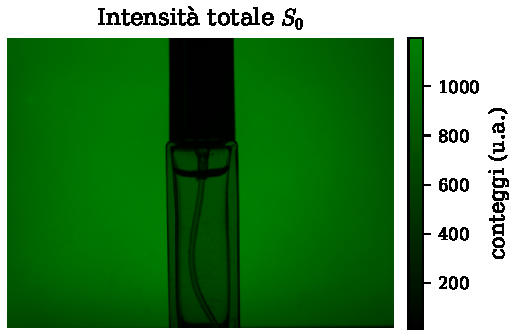
\includegraphics[height=0.205\textwidth]{Images/generated/zucchero/G_S0.pdf}}\hfill
    \subfloat[Canale B ($\lambda_\mathrm{eff} \approx \SI{466}{\nano\meter}$)]{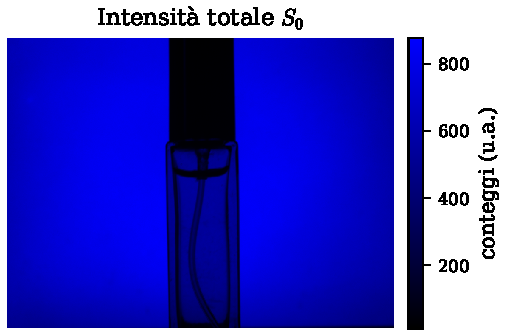
\includegraphics[height=0.205\textwidth]{Images/generated/zucchero/B_S0.pdf}}
    \caption{Mappe di intensità $S_0$ della soluzione di saccarosio sui tre canali del sensore. Si distinguono la boccetta con la soluzione e la cannuccia in plastica impiegata nella preparazione, che introduce una birifrangenza da stress propria visibile localmente nelle mappe di polarizzazione.}
    \label{fig:zucchero_s0}
\end{figure}

La rotazione ottica è piccola, dell'ordine di pochi gradi, e la regione utile della soluzione va distinta dallo sfondo e dai contributi spuri della cannuccia e delle pareti di vetro della boccetta; le eventuali tensioni residue del vetro introdurrebbero peraltro una birifrangenza locale, ossia $\delta \neq 0$, e non una rotazione uniforme dell'AoLP, e non possono quindi mimare l'attività ottica. La stima viene quindi affidata alla procedura di clustering non parziale descritta nella \cref{sec:umap_clustering}, applicata questa volta all'angolo di polarizzazione lineare: l'embedding UMAP dei descrittori di Stokes viene segmentato con HDBSCAN, e il cluster vincente (quello che combina dimensione apprezzabile, bassa dispersione angolare interna e distanza angolare significativa dal cluster dominante dello sfondo) identifica i pixel della soluzione, restituendone l'AoLP mediano, il cui modulo $\tilde\psi_{\mathrm{win}} = |\mathrm{AoLP}|$ quantifica la rotazione ottica. La procedura è ripetuta sui tre canali (\cref{fig:zucchero_winner_r,fig:zucchero_winner_g,fig:zucchero_winner_b}), fornendo tre stime indipendenti alle rispettive lunghezze d'onda; la deviazione mediana assoluta dell'AoLP entro il cluster vincente è inferiore a $0{,}5^\circ$ su tutti i canali.

\begin{figure}[H]
    \centering
    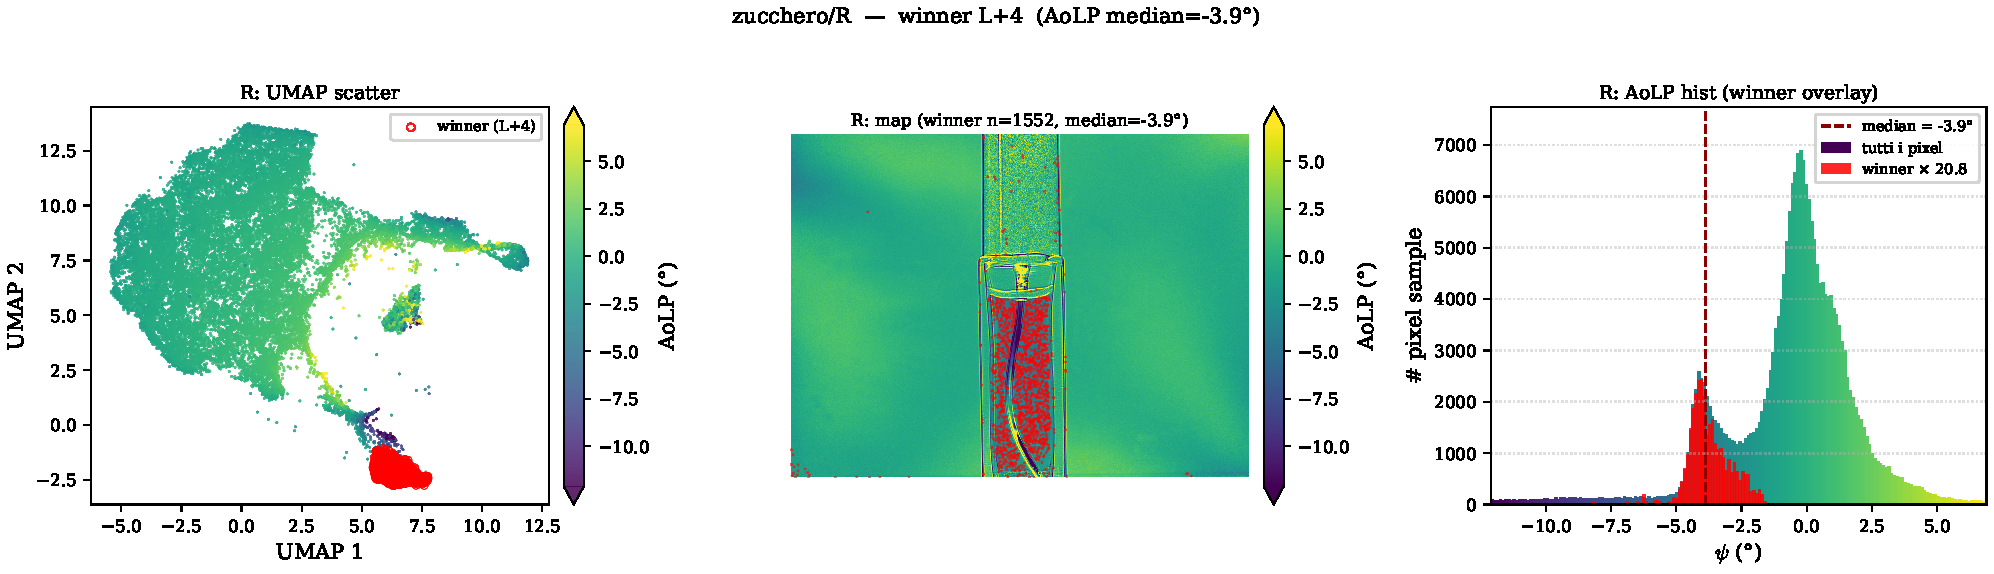
\includegraphics[width=\textwidth]{Images/generated/zucchero/R_aolp_winner.pdf}
    \caption{Identificazione del cluster vincente sul canale rosso: embedding UMAP colorato per AoLP (sinistra), mappa spaziale con il cluster della soluzione evidenziato (centro) e istogramma dell'AoLP (destra). La mediana del cluster vincente è $\mathrm{AoLP} = -3{,}95^\circ$ (rotazione destrogira), corrispondente a una rotazione ottica di modulo $\tilde\psi_{\mathrm{win}} = \SI{3.95}{\degree}$.}
    \label{fig:zucchero_winner_r}
\end{figure}

\begin{figure}[H]
    \centering
    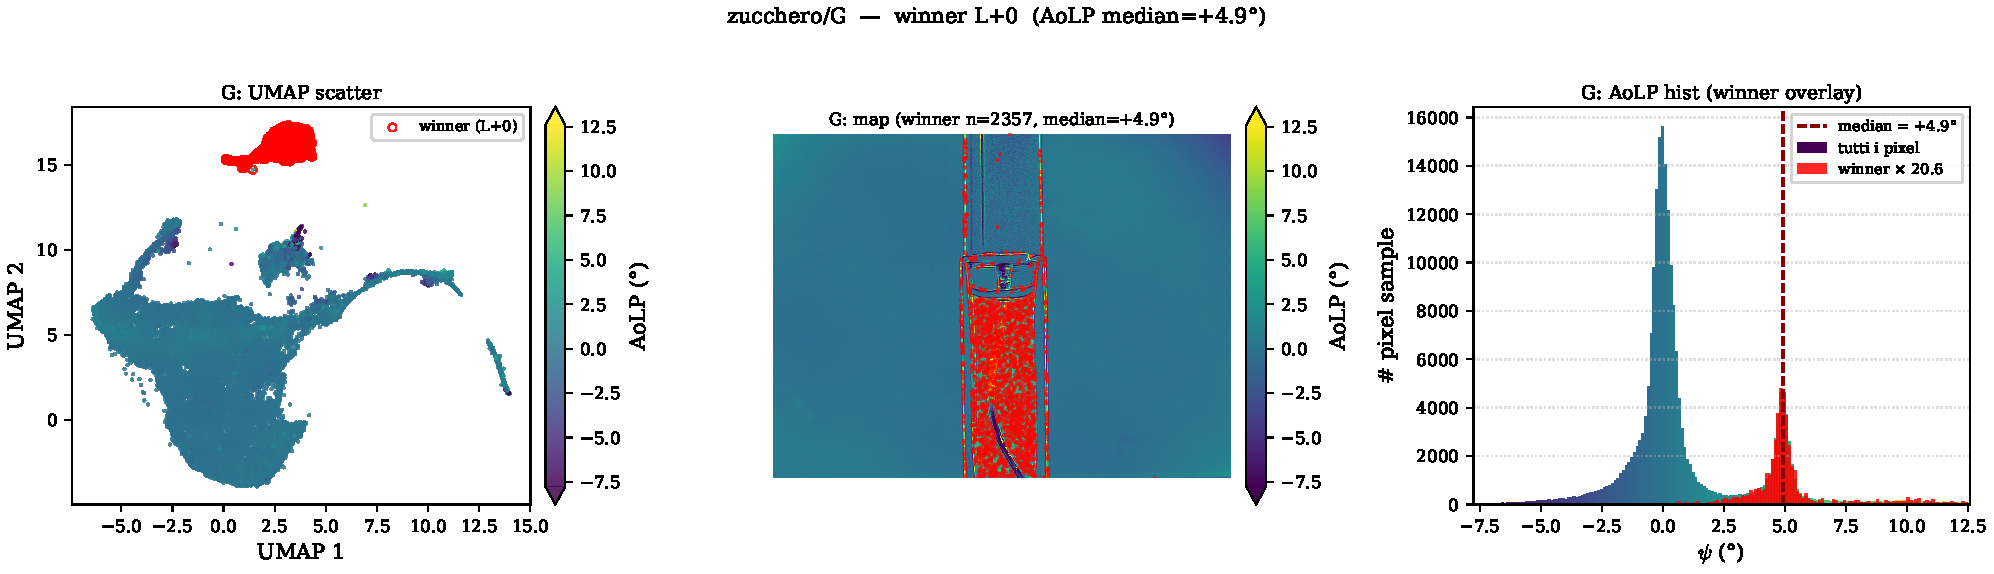
\includegraphics[width=\textwidth]{Images/generated/zucchero/G_aolp_winner.pdf}
    \caption{Cluster vincente sul canale verde, con la stessa struttura a tre pannelli della \cref{fig:zucchero_winner_r}. L'AoLP mediano è $-4{,}92^\circ$, ossia una rotazione di modulo $\tilde\psi_{\mathrm{win}} = \SI{4.92}{\degree}$.}
    \label{fig:zucchero_winner_g}
\end{figure}

\begin{figure}[H]
    \centering
    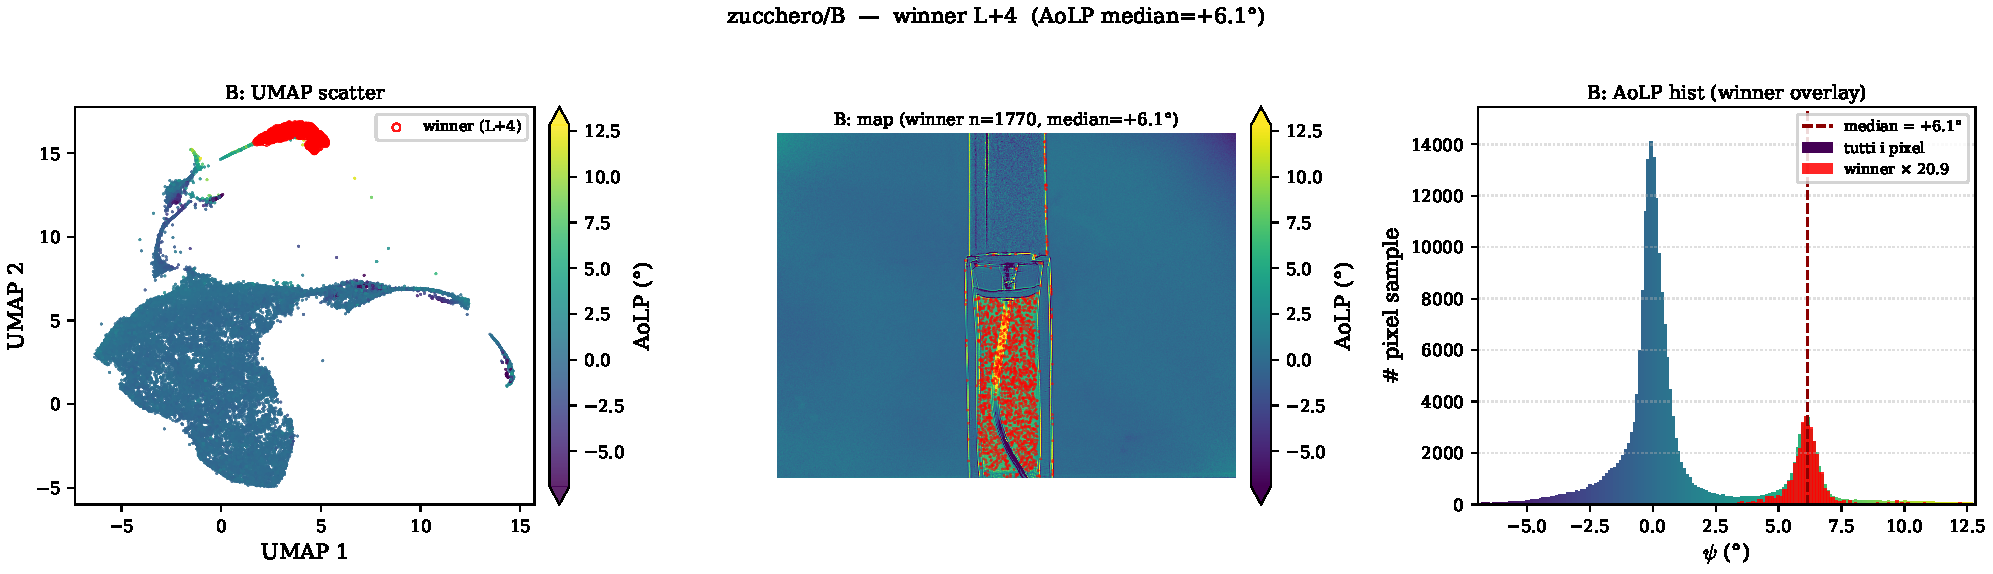
\includegraphics[width=\textwidth]{Images/generated/zucchero/B_aolp_winner.pdf}
    \caption{Cluster vincente sul canale blu, con la stessa struttura a tre pannelli della \cref{fig:zucchero_winner_r}. L'AoLP mediano è $-6{,}12^\circ$, ossia una rotazione di modulo $\tilde\psi_{\mathrm{win}} = \SI{6.12}{\degree}$, la più ampia dei tre canali.}
    \label{fig:zucchero_winner_b}
\end{figure}

La rotazione cresce in modulo al diminuire della lunghezza d'onda, da $\SI{3.95}{\degree}$ al rosso a $\SI{6.12}{\degree}$ al blu, manifestazione della dispersione rotatoria ottica. Il fit con il modello di Drude semplificato, eseguito sull'AoLP mediano con il proprio segno, $\mathrm{AoLP}(\lambda) = k/\lambda^2$ (\cref{fig:zucchero_fit}), restituisce $k = (-1{,}390 \pm 0{,}056)\cdot10^{6}~\si{\degree\nano\meter\squared}$ (errore standard statistico) con $R^2 = 0{,}90$, coerente con $\psi(\lambda) = |k|/\lambda^2$: il modulo di $k$ descrive la dispersione rotatoria, il segno negativo la rotazione destrogira. Il rapporto fra i moduli agli estremi spettrali, $|\psi_B|/|\psi_R| = 6{,}12/3{,}95 = 1{,}55$, è inferiore al rapporto $(\lambda_R/\lambda_B)^2 = 1{,}80$ atteso dal modello $1/\lambda^2$ puro: la dispersione misurata è più piatta della legge inversa quadratica, con uno scostamento che cresce in modo regolare verso le lunghezze d'onda corte. La risonanza ultravioletta del saccarosio non può esserne la causa, poiché renderebbe la dispersione più ripida della legge $1/\lambda^2$, non più piatta; l'appiattimento è quindi da attribuire ai residui sistematici della misura, crescenti verso il blu dove il rapporto segnale-rumore peggiora, e si riflette coerentemente nella lieve decrescita monotona delle stime di concentrazione per canale (\cref{tab:zucchero_conc}).

\begin{figure}[H]
    \centering
    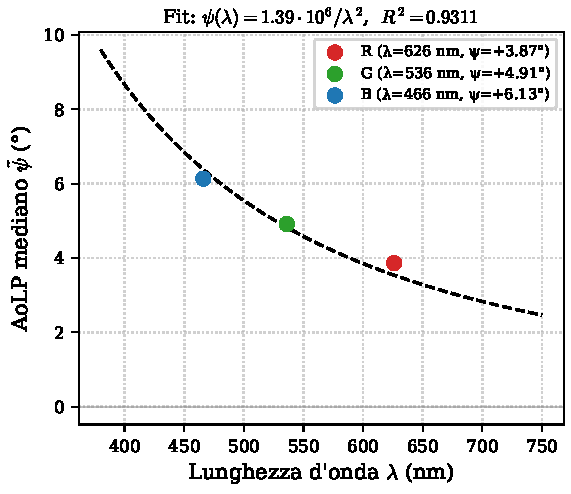
\includegraphics[width=0.55\textwidth]{Images/generated/zucchero/aolp_lambda_fit.pdf}
    \caption{Fit di dispersione rotatoria $\mathrm{AoLP}(\lambda) = k/\lambda^2$ (modello di Drude semplificato, con segno) sull'AoLP mediano del cluster vincente. I punti colorati sono l'AoLP per canale alle rispettive $\lambda_\mathrm{eff}$, con segno negativo coerente con il carattere destrogiro del saccarosio; la curva tratteggiata è il fit non lineare ai minimi quadrati.}
    \label{fig:zucchero_fit}
\end{figure}

La rotazione misurata permette una stima della concentrazione tramite la legge di Biot, $\psi = [\alpha]_\lambda\,L\,c$, dove $[\alpha]_\lambda$ è il potere rotatorio specifico del saccarosio, $L$ il cammino ottico e $c$ la concentrazione in massa per unità di volume. Le misure sono state condotte a temperatura ambiente, non registrata: la dipendenza termica del potere rotatorio del saccarosio è debole, e la sua variazione su pochi gradi attorno alla temperatura di riferimento resta ampiamente al di sotto degli scarti osservati fra i canali. Il valore tabulato alla riga D del sodio, $[\alpha]_{589} = +66{,}5~\si{\degree}\,\si{\milli\liter}\,\si{\gram}^{-1}\,\si{\deci\meter}^{-1}$, viene riportato alle lunghezze d'onda di lavoro tramite lo stesso scaling di Drude, $[\alpha]_\lambda = [\alpha]_{589}\,(589/\lambda)^2$. Invertendo la legge di Biot con $L = \SI{0.13}{\deci\meter}$ si ottengono le tre stime di concentrazione raccolte nella \cref{tab:zucchero_conc}.

\begin{table}[H]
    \centering
    \caption{Rotazione ottica del cluster vincente, potere rotatorio specifico riportato alla lunghezza d'onda di lavoro e concentrazione stimata via legge di Biot per la soluzione di saccarosio ($L = \SI{13}{\milli\meter}$).}
    \label{tab:zucchero_conc}
    \begin{tabular}{lcccc}
        \hline
        \textbf{Canale} & $\lambda_\mathrm{eff}$ [\si{\nano\meter}] & $\tilde\psi_{\mathrm{win}}$ [\si{\degree}] & $[\alpha]_\lambda$ [\si{\degree}\,\si{\milli\liter}\,\si{\gram}$^{-1}$\,\si{\deci\meter}$^{-1}$] & $c$ [\si{\gram\per\milli\liter}] \\
        \hline
        Rosso & 626 & $3{,}95$ & $58{,}9$  & $0{,}52$ \\
        Verde & 536 & $4{,}92$ & $80{,}3$  & $0{,}47$ \\
        Blu   & 466 & $6{,}12$ & $106{,}2$ & $0{,}44$ \\
        \hline
    \end{tabular}
\end{table}

Le tre stime si collocano entro circa il $\pm 9\%$ attorno al valore medio $c_\mathrm{ott} \approx \SI{0.47}{\gram\per\milli\liter}$, con la decrescita monotona dal rosso al blu già ricondotta ai residui sistematici della misura. La consistenza della concentrazione ricavata indipendentemente da tre canali colore distinti, ciascuno con la propria correzione di dispersione, è il risultato significativo della misura: il sistema recupera un valore quantitativo coerente combinando la legge di Biot con la dispersione rotatoria. La soluzione è stata preparata mescolando zucchero e acqua senza un controllo gravimetrico accurato, per cui non è disponibile un riferimento di concentrazione affidabile con cui validare l'accuratezza assoluta; il valore ricavato è comunque del tutto plausibile per una soluzione zuccherina concentrata e dimostra la capacità del polarimetro di misurare l'attività ottica in modo quantitativo e spettralmente coerente.

\subsection{Trave a sbalzo}
\label{subsec:risultati_cantilever}

La fotoelasticità è la comparsa di birifrangenza in un materiale otticamente isotropo sottoposto a sforzo meccanico: gli assi della birifrangenza indotta si allineano con le direzioni principali dello sforzo e il ritardo è proporzionale alla differenza degli sforzi principali. Il campione è una barra in materiale polimerico trasparente a sezione quadrata di lato $\SI{8}{\milli\meter}$, vincolata a un'estremità come trave a sbalzo e caricata all'estremità libera con un parallelepipedo metallico di massa circa $\SI{900}{\gram}$, corrispondente a una forza applicata dell'ordine di $\SI{9}{\newton}$; la distanza fra il punto di applicazione del carico e l'estremo del vincolo è di circa $\SI{73}{\milli\meter}$. Questi dati geometrici sono riportati a titolo di contesto e non vengono impiegati per un'analisi quantitativa. Le acquisizioni sono state ripetute nelle due condizioni di trave scarica (\texttt{barraoff\_v2}) e sotto carico (\texttt{barraon\_v2}).

L'orientazione del campione condiziona fortemente la leggibilità del segnale. La barra è stata posizionata con il proprio asse longitudinale parallelo alla direzione di polarizzazione della luce incidente; poiché in una trave inflessa lo sforzo principale è diretto lungo l'asse, gli assi della birifrangenza indotta risultano quasi paralleli (o perpendicolari) alla polarizzazione di ingresso. In questa configurazione l'angolo $\alpha$ fra asse veloce e polarizzazione è prossimo a $0^\circ$, e la conversione della polarizzazione lineare in componente circolare, governata dal fattore $\sin 2\alpha\,\sin\delta$ (\cref{eq:s3_ritardatore}), è fortemente soppressa. La stessa condizione rende degenere l'estrazione della ritardanza, che il peso di stabilità della pipeline (\cref{subsec:ambiguita_numeriche}) spinge verso zero quando $\sin^2 2\alpha \to 0$. Gli effetti birifrangenti sono perciò poco evidenti e l'estrazione di grandezze quantitative non è affidabile. Anche disponendo della geometria della barra, il modulo elastico del polimero e il coefficiente fotoelastico del materiale non sono noti, e l'orientazione sfavorevole rispetto alla polarizzazione sopprime comunque il segnale: per queste ragioni non si tenta una stima del campo di sforzo e l'analisi resta qualitativa, concentrandosi sulla componente $S_3$.

\begin{figure}[H]
    \centering
    \subfloat[Canale R ($\lambda_\mathrm{eff} \approx \SI{626}{\nano\meter}$)]{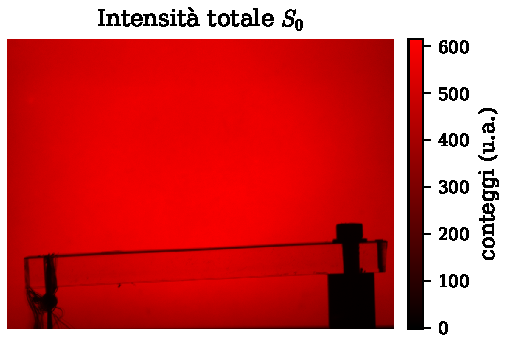
\includegraphics[height=0.205\textwidth]{Images/generated/barraon_v2/R_S0.pdf}}\hfill
    \subfloat[Canale G ($\lambda_\mathrm{eff} \approx \SI{536}{\nano\meter}$)]{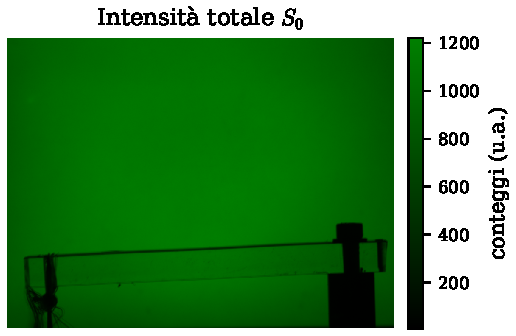
\includegraphics[height=0.205\textwidth]{Images/generated/barraon_v2/G_S0.pdf}}\hfill
    \subfloat[Canale B ($\lambda_\mathrm{eff} \approx \SI{466}{\nano\meter}$)]{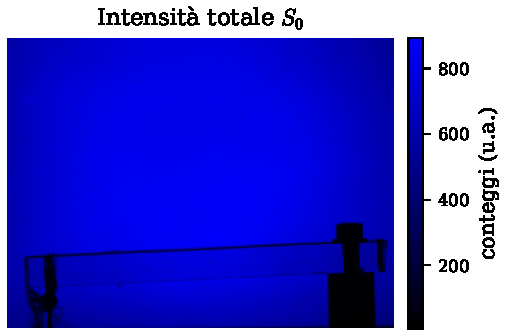
\includegraphics[height=0.205\textwidth]{Images/generated/barraon_v2/B_S0.pdf}}
    \caption{Mappe di intensità $S_0$ della trave a sbalzo sotto carico sui tre canali del sensore. Si distinguono il corpo della barra, il vincolo a sinistra e il supporto destro impiegato come riferimento per la registrazione.}
    \label{fig:barra_s0}
\end{figure}

Per isolare la variazione indotta dal carico, le acquisizioni con e senza peso vanno riportate alla stessa geometria: la trave sotto carico si flette e il campo di vista subisce un piccolo spostamento rigido fra le due riprese. Si applica perciò la procedura descritta nella \cref{sec:fotoelasticita}: un allineamento globale per correlazione di fase calcolato sul solo supporto destro, dove la flessione è trascurabile, seguito da una deformazione colonna-per-colonna che riporta la centerline della trave carica su quella della trave scarica. La mappa differenziale $\Delta S_3 = S_3^{\mathrm{on,\,warped}} - S_3^{\mathrm{off}}$, calcolata indipendentemente sui tre canali (\cref{fig:barra_ds3}), elimina la componente comune dovuta all'illuminazione e alla geometria, isolando il solo contributo dello stato di sforzo.

\begin{figure}[H]
    \centering
    \subfloat[Canale R]{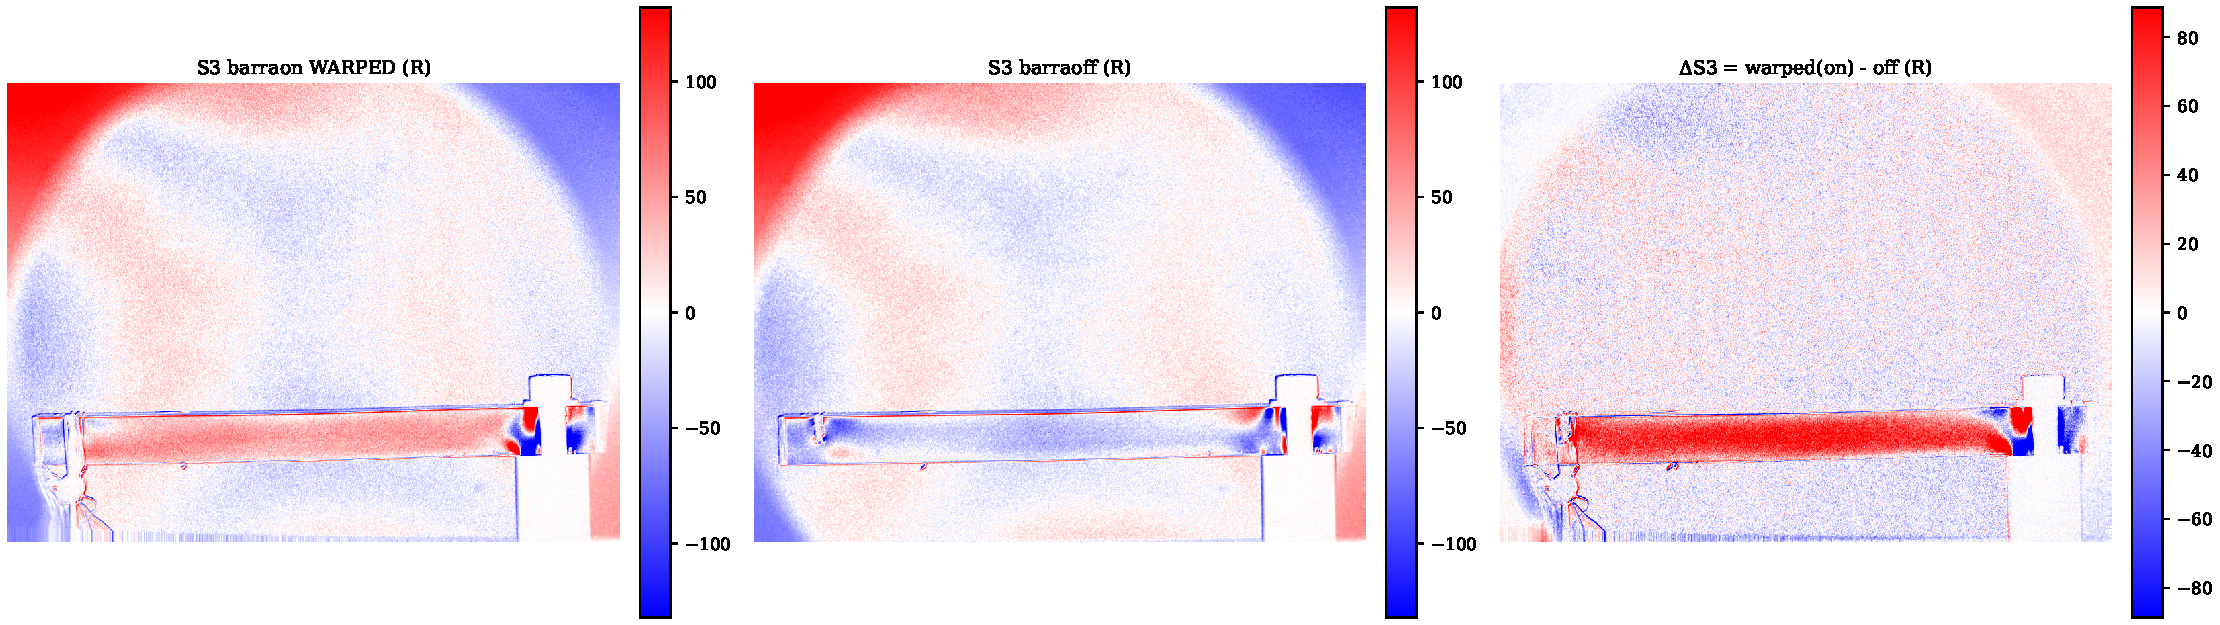
\includegraphics[height=0.205\textwidth]{Images/generated/barraon_v2/R_diff_s3_warped.pdf}}\hfill
    \subfloat[Canale G]{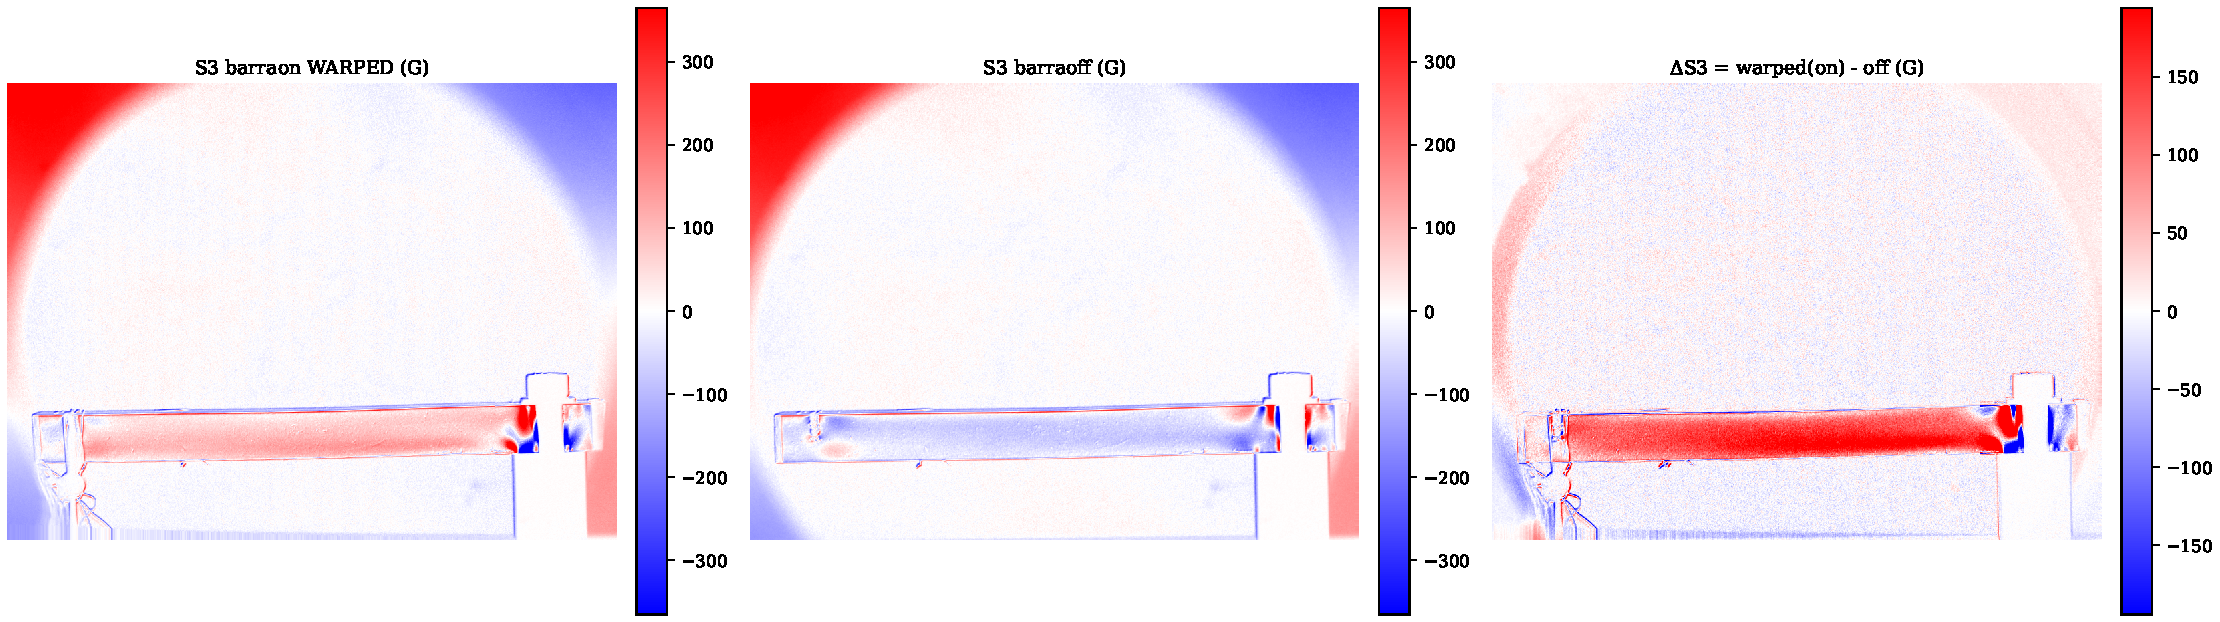
\includegraphics[height=0.205\textwidth]{Images/generated/barraon_v2/G_diff_s3_warped.pdf}}\hfill
    \subfloat[Canale B]{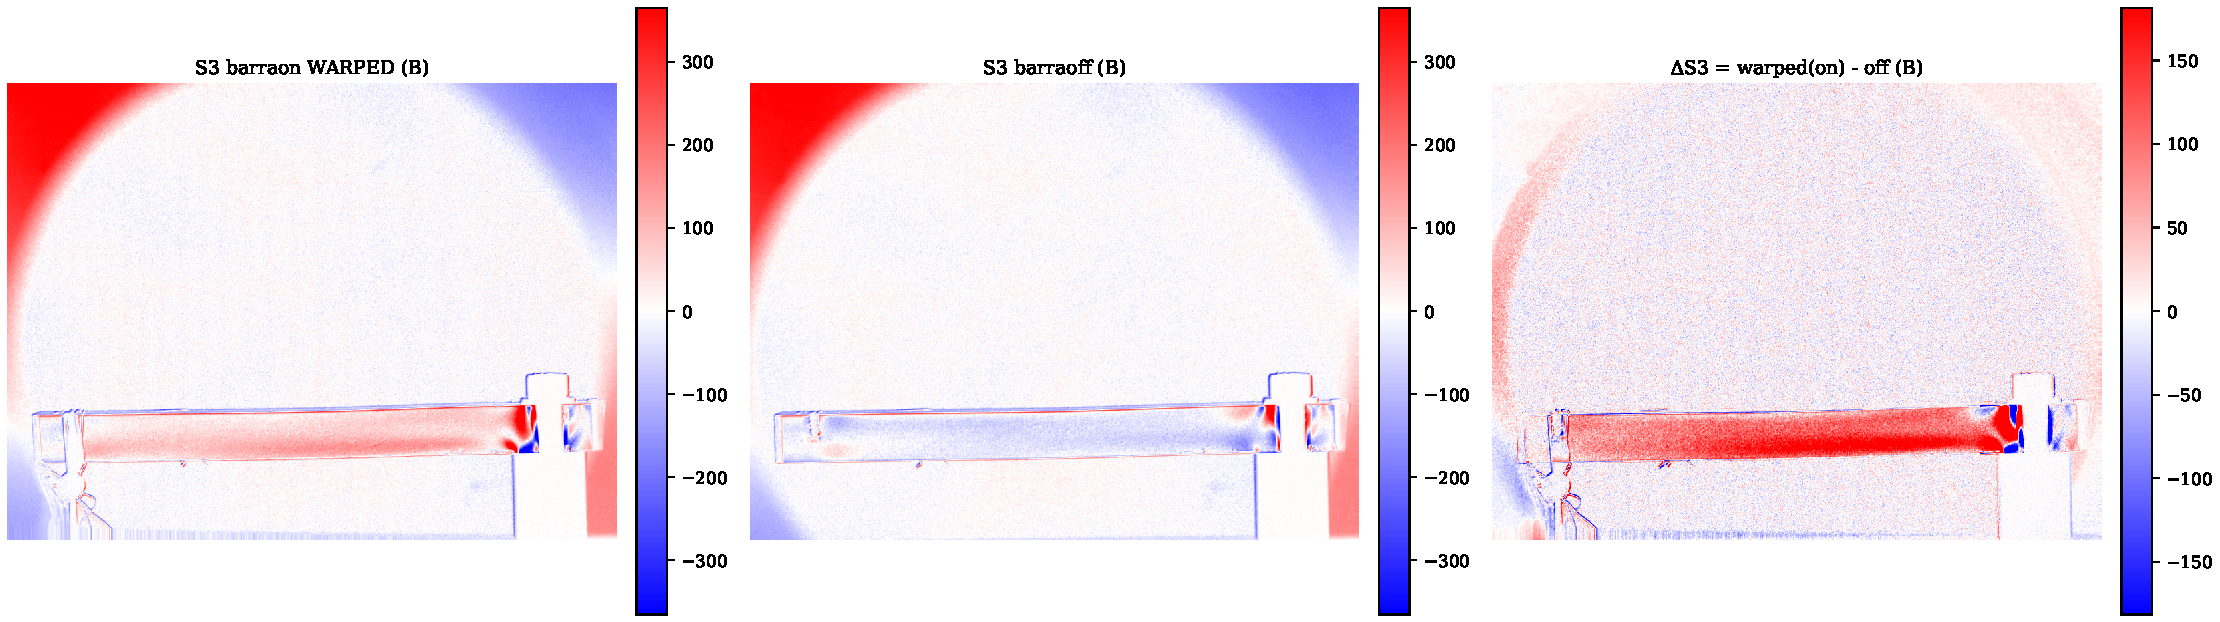
\includegraphics[height=0.205\textwidth]{Images/generated/barraon_v2/B_diff_s3_warped.pdf}}
    \caption{Mappa differenziale $\Delta S_3 = S_3^{\mathrm{on,\,warped}} - S_3^{\mathrm{off}}$ fra trave carica e scarica, sui tre canali del sensore, dopo registrazione e deformazione colonna-per-colonna. Il differenziale isola il contributo della birifrangenza indotta dal carico.}
    \label{fig:barra_ds3}
\end{figure}

% TODO (utente): inserire la lettura qualitativa specifica delle mappe DeltaS3 (dove compare il segnale sotto carico, segno, eventuale localizzazione presso il vincolo). Confine di interpretazione umana: la descrizione spaziale delle mappe spetta all'utente.
La mappa differenziale evidenzia, sia pur debolmente, la comparsa di un segnale $S_3$ associato al carico, assente nella configurazione scarica: il confronto conferma in via qualitativa la natura fotoelastica del campione e la sensibilità del polarimetro alla birifrangenza indotta da sforzo, pur nei limiti imposti dall'orientazione sfavorevole della barra rispetto alla polarizzazione incidente.

% ---------------------------------------------------------------------------
\section{Discussione}
\label{sec:discussione}

I risultati presentati nelle sezioni precedenti dimostrano che il sistema è in grado di ricostruire il vettore di Stokes completo con risoluzione spaziale bidimensionale, di misurare ritardanza e asse veloce su campioni macroscopici, e di distinguere fenomeni polarimetrici di natura diversa (birifrangenza, attività ottica, fotoelasticità) con un apparato il cui costo complessivo, escluso lo smartphone, è inferiore a 100\,\texteuro.

Una stima rigorosa dell'incertezza di misura esula dalle possibilità di questo lavoro: quantificarla richiederebbe una calibrazione dello strumento contro campioni a ritardanza nota e con incertezza certificata, riferimenti non disponibili per un prototipo che non ha ancora ricevuto una caratterizzazione metrologica. In assenza di tali standard, l'accuratezza può essere valutata soltanto per confronto con le previsioni teoriche sui campioni di validazione, e gli scarti osservati si collocano nell'ordine di pochi gradi. Le incertezze riportate sui parametri dei fit (la pendenza per strato del nastro e i prefattori di dispersione) sono errori standard puramente statistici, ricavati dai residui dei fit stessi: quantificano la riproducibilità interna dei dati, non l'accuratezza assoluta, che resta dominata dai contributi sistematici discussi in questa sezione. La lamina quarto d'onda, il cui ritardo misurato è stato confrontato con la legge di dispersione di un ritardatore a singolo ordine (\cref{subsec:risultati_qw}), ne è l'esempio più diretto: lo scarto è di pochi gradi al rosso, prossimo al punto di design, mentre l'eccedenza che cresce verso il blu ingloba anche il contributo fisico della dispersione del materiale, che il riferimento puramente geometrico per costruzione non modella. Tali valori vanno intesi come ordine di grandezza dell'accordo con la teoria, non come una barra d'errore calibrata.

Lo scarto non si distribuisce in modo uniforme fra le grandezze ricostruite, e la gerarchia osservata riflette la lunghezza della catena di misura che ciascuna richiede. L'angolo di polarizzazione lineare e il grado di polarizzazione discendono direttamente dai parametri di Stokes lineari $S_0$, $S_1$ e $S_2$, estratti dal sistema sovradeterminato delle trentasei acquisizioni angolari, e risultano perciò le grandezze più stabili. La ritardanza richiede invece la determinazione di $S_3$, e con essa le due acquisizioni aggiuntive con lamina $\lambda/4$, la correzione cromatica del ritardo della lamina e l'azzeramento dell'ellitticità residua sulla sfera di Poincaré; la catena più lunga, sommata all'ambiguità di avvolgimento modulo $360^\circ$ per i campioni ad alta ritardanza, rende $\delta$ la quantità intrinsecamente meno precisa, in accordo con la maggiore sensibilità del suo calcolo alle approssimazioni discusse di seguito.

% TODO: check (coerenza downsample f=4 sistemata da AI 2026-05-21)
Il principale compromesso è introdotto dal downsampling: con il fattore $f = 4$ adottato in questo lavoro la risoluzione di analisi resta di circa $6 \cdot 10^5$ pixel ($912 \times 684$), sufficiente per i campioni macroscopici considerati ma tale da rendere irrisolvibili strutture più piccole di qualche centinaio di micrometri, corrispondendo ciascun pixel di analisi a circa \SI{114}{\micro\meter} al piano del campione (\cref{sec:sensore}). Per i campioni macroscopici analizzati questa limitazione non è stata rilevante, ma applicazioni su scala microscopica richiederebbero un'elaborazione a blocchi o su GPU.

Un secondo limite è l'approssimazione monocromatica: l'assegnazione di una singola lunghezza d'onda effettiva a ciascun canale colore ignora la larghezza di banda dei filtri Bayer, che si estende su diverse decine di nanometri. Per campioni con forte dispersione, la misura rappresenta una media pesata sulla banda; una caratterizzazione più fine richiederebbe filtri passa-banda stretti o una sorgente monocromatica.

La sensibilità alla correzione cromatica di $S_3$ è un terzo fattore: sebbene il ritardo $\delta_a(\lambda)$ della lamina analizzatore sia calibrato direttamente dai dati (\cref{sec:calibrazione_s3}) e non assunto da un modello di materiale, il fattore $1/\sin\delta_a(\lambda)$ cresce verso il blu, dove diventa più sensibile sia agli errori residui di calibrazione sia al rumore di $S_3$. Al canale rosso la correzione è prossima all'unità e quindi robusta a ogni scelta di modello, il che spiega la scelta del rosso come canale predefinito per l'analisi.

Un quarto fattore, specifico della ritardanza, è l'allineamento geometrico delle lamine. L'inserimento manuale della lamina $\lambda/4$ analizzatore e delle lamine campione non garantisce un'incidenza esattamente normale, e un'inclinazione residua di pochi gradi altera il cammino ottico e la birifrangenza efficace, con una variazione frazionaria del ritardo che cresce quadraticamente con l'angolo. Per una lamina a basso ordine l'effetto è trascurabile, dell'ordine del decimo di grado per inclinazioni di alcuni gradi, e la calibrazione di $S_3$, fondata sulla $\lambda/4$ a ordine zero, ne è di fatto immune; ma poiché la variazione si applica al ritardo \emph{totale}, su un campione ad alto ritardo accumulato essa cresce in proporzione, fino ad alcuni gradi sul valore avvolto oltre i $\SI{1500}{\degree}$ del nastro multistrato, e contribuisce allo scarto residuo osservato su tali campioni.

Il confronto con le principali classi di strumentazione polarimetrica commerciale (\cref{tab:confronto}) colloca il sistema in una posizione intermedia. Le telecamere a divisione del piano focale offrono imaging di polarizzazione a costo contenuto, ma rinunciano alla componente circolare $S_3$; i sistemi a immagine full-Stokes o di matrice di Mueller, capaci della stessa misura completa ottenuta in questo lavoro, hanno invece costi di due o tre ordini di grandezza superiori. Il prototipo scambia accuratezza assoluta e risoluzione spettrale con costo, portabilità e accessibilità, e risulta particolarmente adatto a contesti didattici e a misure esplorative, dove la rapidità di setup e il basso costo compensano le limitazioni in precisione.

\begin{table}[H]
    \centering
    \footnotesize
    \setlength{\tabcolsep}{4pt}
    \caption{Confronto fra il polarimetro proposto e le principali classi di strumentazione polarimetrica commerciale (polarimetro di Stokes puntuale, telecamera DoFP, sistemi a immagine full-Stokes o di matrice di Mueller). Il costo del sistema proposto esclude lo smartphone. Prezzi e accuratezze sono valori indicativi di listino o di specifica (2024--2026); per il prototipo l'accuratezza è l'ordine di grandezza dello scarto dalle previsioni teoriche, in assenza di calibrazione.}
    \label{tab:confronto}
    \begin{tabularx}{\textwidth}{@{}>{\raggedright\arraybackslash}p{2.6cm} *{4}{>{\raggedright\arraybackslash}X}@{}}
        \hline
        \textbf{Caratteristica} & \textbf{Questo lavoro} & \textbf{Polarimetro puntuale} & \textbf{Camera DoFP} & \textbf{Imaging full-Stokes / Mueller} \\
        \hline
        Grandezza misurata & $S_0$--$S_3$ & $S_0$--$S_3$ & $S_0$--$S_2$ (lineare) & $S_0$--$S_3$ / Mueller \\
        Risoluzione spaziale & Sì, 2D & No (puntuale) & Sì (snapshot) & Sì, 2D \\
        Risoluzione spettrale & Banda larga (Bayer) & Mono.\ o a banda & Banda larga (Bayer) & Mono.\ o iperspettr. \\
        Misura di $S_3$ & Sì (lamina $\lambda/4$) & Sì & No & Sì \\
        Automazione & Manuale & Motorizzata & Snapshot & Motorizz./attiva \\
        Accuratezza tipica & $\sim 1$--$5^\circ$ & $\sim 0{,}25^\circ$ & $< 0{,}5^\circ$ & $\lesssim 0{,}1^\circ$ \\
        Costo indicativo & $<100$\,\texteuro & $3$--$6$\,k\texteuro & $2$--$2{,}5$\,k\texteuro & $10^4$--$10^5$\,\texteuro \\
        \hline
    \end{tabularx}
\end{table}
